%==============================================================================
% Predicting Quarterly Airbnb Booking Demand in New York City
% Technical Report -- IEEEtran journal source
%
% Compile with:  pdflatex main  ->  bibtex main  ->  pdflatex main  ->  pdflatex main
% (or upload the whole paper/ folder to Overleaf and press Recompile)
%
% This revision migrates the original 2016 Kaggle-cloned-competition study to
% the open Inside Airbnb data for New York City (2025-2026), keeping the same
% modelling philosophy (leakage-safe pipelines, tree ensembles, a convex
% weighted blend) while re-deriving every feature, target, and result from
% scratch under a strict historical-only feature window.
%==============================================================================
\documentclass[journal]{IEEEtran}

\usepackage{amsmath,amssymb,amsfonts}
\usepackage{graphicx}
\usepackage{textcomp}
\usepackage{booktabs}
\usepackage{url}
\usepackage[T1]{fontenc}
\usepackage[utf8]{inputenc}
\usepackage{xcolor}
\graphicspath{{figures/}}

\hyphenation{op-tical net-works semi-conduc-tor}

\begin{document}

\title{Predicting Quarterly Airbnb Booking Demand in New York City with
Tree-Based Ensembles and a Weighted Model Blend}

\author{Muhammed~Ali~Bak{\i}r~and~Mahmut~Sami~Ba\c{s}kal%
\thanks{Computer Engineering Department, Abdullah G\"ul University,
Kayseri, T\"urkiye.
E-mail: muhammedali.bakir@agu.edu.tr; mahmutsami.baskal@agu.edu.tr.}%
\thanks{This report describes an independent follow-up study; the pipeline,
experiments, and results reported here are the work of M.\ S.\ Ba\c{s}kal.}}

\markboth{Technical Report}%
{Bak{\i}r and Ba\c{s}kal: Predicting Quarterly Airbnb Booking Demand in NYC}

\maketitle

\begin{abstract}
Forecasting how much a short-term rental will be booked is a useful but
difficult problem for both hosts and the platforms that connect them with
guests. This report is a follow-up to an earlier study of ours that used a
fixed, academic snapshot of 2016 New York City Airbnb data; here we migrate the
same modelling philosophy to the publicly available Inside Airbnb data for New
York City, using the July 2025 -- March 2026 window. The task is to predict,
for roughly 36{,}000 active properties, the number of nights blocked (i.e.,
effectively booked) during the first quarter of 2026 (January--March, 90 days),
using only information available through the end of 2025 -- no feature is ever
built from 2026 data, which is reserved exclusively for deriving the target.
Starting from a static listings snapshot and six monthly calendar/review
histories (July--December 2025, jointly over 79 million listing-day rows), we
engineered a flat matrix of 206 features per property covering calendar
occupancy dynamics at several time horizons, recency and trajectory signals,
review velocity, price and revenue proxies, host attributes, amenities and
title keywords, and neighbourhood/geo-cluster context. We compared nine model
configurations -- Linear Regression, Random Forest, Gradient Boosting, three
XGBoost variants, a PyTorch Multi-Layer Perceptron (MLP), LightGBM, and CatBoost
-- inside leakage-safe scikit-learn pipelines, tuning the boosted trees with a
randomized search that uses fold-level early stopping. Our best single model,
a tuned XGBoost regressor, reached a 5-fold cross-validation MSE of 295.7 on
the development set, and a convex (SLSQP) weighted blend of all nine models
lowered the out-of-fold MSE to 290.1, a gain we verify with a paired
significance test ($t=7.27$, $p=3.7\times10^{-13}$). We also implement, rather
than merely propose, a two-stage hurdle model (a classifier for ``will this
property see any activity at all'' followed by a regressor for the positive
counts) motivated by a residual analysis on the bounded $[0,90]$ target, and we
report an incremental ablation isolating how much of the final error reduction
comes from feature engineering, target encoding, tree ensembling, and blending,
respectively. On a held-out local test split (20\% of the data, never touched
during model selection or tuning) the final blend reaches an MSE of 286.1.
\end{abstract}

\begin{IEEEkeywords}
Airbnb, demand forecasting, regression, ensemble learning, XGBoost, LightGBM,
CatBoost, random forest, multi-layer perceptron, model blending, target
encoding, hurdle model, constrained optimization, mean squared error, feature
engineering.
\end{IEEEkeywords}

%==============================================================================
\section{Introduction}
\IEEEPARstart{O}{ver} the last ten years, peer-to-peer (P2P) accommodation
platforms have reshaped the way people travel and the way property owners earn
money from their homes. Airbnb is the most visible example of this shift, with
millions of active listings spread across more than a hundred thousand cities
worldwide \cite{adamiak2018}. For a platform of that size, two questions tend
to dominate the business: what is a fair price for a given listing, and how
much demand will that listing actually receive over some future period. This
report keeps that second focus, but changes the data foundation: an earlier
version of this study used a fixed, academic snapshot of 2016 New York City
Airbnb data distributed for a course competition; here we migrate the same
pipeline philosophy to the publicly available Inside Airbnb data
\cite{insideairbnb}, re-deriving every feature, target, and result on a
2025--2026 window.

Being able to predict demand a quarter in advance is valuable for several
practical reasons. A host who knows that the next three months will be busy can
schedule cleaning and maintenance, raise prices for the high-demand weeks, or
decide that it is worth hiring help. The platform, on its side, can plan
customer-support capacity, target marketing toward listings that look like they
will be under-booked, and give hosts better pricing recommendations. The
trouble is that demand is the result of many interacting factors---the property
type and capacity, the neighbourhood, seasonality, the host's responsiveness,
the review history, and how aggressively the price moves during the period.
Classical linear models have been used for this kind of accommodation data
\cite{gunter2018,wang2017}, but a fairly consistent finding in the recent
literature is that machine-learning models, and tree-based ensembles in
particular, tend to do better on the mixed numerical and categorical tables
that describe short-term rentals \cite{tang2024,camatti2024,kalehbasti2019}.

Concretely, the task is to predict, for roughly 36{,}000 active New York City
properties, the total number of nights blocked (effectively booked) during the
first quarter of 2026 (January, February, and March). Because that quarter
contains 90 days, the target is an integer between 0 and 90, and we score it
purely by Mean Squared Error, matching the metric used throughout the earlier
2016-data study. A design decision that shapes every part of this report is a
strict temporal boundary: every engineered feature is built exclusively from
data observed through the end of December 2025 (the second half, or ``H2,'' of
2025); the 2026 calendar snapshots are used only to construct the target,
never as a predictor. This mirrors an honest forecasting deployment, where the
model would have to make its prediction before any 2026 data existed at all.

This report is organized as follows. Section~\ref{sec:lit} reviews the most
relevant prior work on Airbnb prediction, decision-tree ensembles,
hyper-parameter tuning, and preprocessing, and adds a short mathematical
argument for why linear models struggle with a zero-inflated bounded target.
Section~\ref{sec:settings} describes the project setting: the problem statement
and the dataset. Section~\ref{sec:method} gives the full methodology and
defines every custom component---the target encoder, the search loop, the MLP,
and the blend---with explicit equations. Section~\ref{sec:results} presents our
results, an incremental ablation, a significance test for the blend, and a
residual analysis on the target boundaries that motivates a two-stage hurdle
model. Section~\ref{sec:changes} discusses the concrete choices that changed in
migrating from the original 2016-data pipeline to the new dataset.
Section~\ref{sec:concl} concludes and lists what we would try next.

%==============================================================================
\section{Literature Review}
\label{sec:lit}
We group the related work into four areas: (A) machine learning for Airbnb
prediction tasks, (B) decision trees and tree-based ensembles, (C)
hyper-parameter tuning and model validation, and (D) data preprocessing and
feature engineering. Most of this review carries over unchanged from the
2016-data study this report follows up on; here we keep the parts that ended
up actually guiding the final solution and trim the ones that did not.

\subsection{Machine Learning for Airbnb Prediction Tasks}
Several studies apply machine learning directly to Airbnb data. Tang, Cheng, and
Zhang \cite{tang2024} worked with listings from Sydney and compared ten
algorithms including Random Forest, Gradient Boosting, and CatBoost for price
prediction. CatBoost gave them the lowest root mean squared error, and the most
influential features were the maximum number of guests, the number of bedrooms,
and whether the room was private or shared. Camatti et al.\ \cite{camatti2024}
ran a comparative analysis of artificial-intelligence and traditional linear
methods on Dutch Airbnb listings, and concluded that tree-based and
neural-network methods overfit less than linear regression, though linear models
are still handy for reading off which predictors matter. Rezazadeh Kalehbasti,
Nikolenko, and Rezaei \cite{kalehbasti2019} predicted New York City Airbnb
prices using property features, host characteristics, and the sentiment of
customer reviews; their best model was a regularized linear model built on
review-text features, but tree models such as Random Forest and Support Vector
Regression were close behind.

Other work looks at demand rather than price, which is closer to our own task.
Siker \cite{siker2018} tackled the Kaggle ``Airbnb New User Bookings'' problem
with XGBoost, and even though the target there (destination country) is
different from ours, the workflow---heavy feature engineering followed by
gradient boosting---matches how most Airbnb-style Kaggle problems are solved in
practice. Chapman, Mohammad, and Villegas \cite{chapman2023} studied dynamic
short-term rental markets and built a pipeline that merged listing, calendar,
and review data; they again found gradient boosting beating linear regression.
Islam et al.\ \cite{islam2022} combined a Latent Dirichlet Allocation topic
model over property descriptions with an XGBoost regressor and improved price
prediction on the San Jose dataset. Two lessons from this group shaped our
project: first, the most useful predictors are usually a mix of structural
features, location, and dynamic calendar/review information; and second,
gradient-boosted trees are a strong default because they cope well with mixed
feature types and missing values.

A recurring theme across these studies is that the engineering choices around the
model often matter more than the model itself. Tang et al.\ \cite{tang2024} and
Islam et al.\ \cite{islam2022} both report that their largest gains came from the
features they constructed---guest capacity and room type in the first case, topic
structure of the listing description in the second---rather than from swapping one
boosting library for another. Kalehbasti et al.\ \cite{kalehbasti2019} similarly
found that review-sentiment features moved their error more than the choice
between a regularized linear model and a tree ensemble. This is consistent with
the broader observation that on tabular problems the ceiling is usually set by how
much signal the practitioner can encode, and it is precisely why we invested most
of our effort in the 150-feature matrix and treated the model comparison as a
secondary, if still important, step. It also explains why a competition with a
fixed, shared dataset is decided largely by feature engineering and validation
discipline rather than by access to a particular algorithm---an observation that
shaped how we allocated our time.

\subsection{Why Linear Models Underfit a Zero-Inflated Bounded Target}
\label{sec:linearcritique}
Beyond the empirical observation that linear regression trails the trees, it is
worth stating \emph{why} in mathematical terms, because the shape of our target
is the crux of the whole problem. Ordinary least squares fits
$\hat y(\mathbf{x}) = \boldsymbol{\beta}^{\top}\mathbf{x}$ by minimizing the
population risk $\mathbb{E}\big[(y-\boldsymbol{\beta}^{\top}\mathbf{x})^{2}\big]$,
whose minimizer is the conditional mean $\mathbb{E}[y\mid\mathbf{x}]$
\emph{restricted to the class of affine functions}. Our target, however, is a
censored count confined to $[0,90]$ with a large probability mass at $0$
(roughly 50\% of the development rows are exactly zero; see
Fig.~\ref{fig:target}). Its true conditional mean is therefore an inherently
nonlinear, saturating function of the covariates: it must flatten to $0$ for
low-demand listings and saturate toward $90$ for high-demand ones. An affine
predictor cannot reproduce those two plateaus---it extrapolates linearly past
both edges, so it produces negative fitted values for the dead listings (which
are then clipped, wasting capacity) and undershoots the busiest ones. Formally,
if $y=\max\!\big(0,\min(90,\ \boldsymbol{\beta}^{\top}\mathbf{x}+\varepsilon)\big)$,
the censoring makes $\mathbb{E}[y\mid\mathbf{x}]$ a \emph{nonlinear} function of
$\mathbf{x}$ even when the latent variable is linear, which is exactly the
limited-dependent-variable setting that motivated Tobit-type estimators
\cite{tobin1958} and, more directly for counts, two-part (hurdle) models.
Earlier price-prediction studies that reported linear baselines
\cite{gunter2018,wang2017} did not face this point mass because price is
continuous and unbounded; demand counts are not, and that is the structural
reason their linear formulations do not transfer to our task. Tree ensembles
sidestep the issue entirely: a regression tree approximates the saturating
conditional mean with axis-aligned piecewise-constant regions, so the $0$ and
$90$ plateaus are simply leaves, and boosting refines the transition region
between them.

\subsection{Modelling Zero-Inflated and Count Targets}
\label{sec:zeroinflated}
Our target is a bounded count with a large spike at zero, and the statistics
literature offers a dedicated family of models for exactly this shape. A plain
Poisson regression assumes the conditional mean equals the conditional variance,
which is violated here because the zero spike and the upper-bound pile-up make
the data strongly over-dispersed. Negative-binomial regression relaxes that
equal-mean-variance assumption but still does not account for the excess of
structural zeros. Two model classes target the zeros directly: zero-inflated
models (e.g.\ zero-inflated Poisson, ZIP) mix a point mass at zero with a count
distribution, and \emph{hurdle} (two-part) models first decide whether the count
is positive and then model the positive counts separately. Censored-regression
estimators such as Tobit \cite{tobin1958} instead treat the bound itself as the
generative mechanism. We did not adopt these parametric estimators directly---
gradient-boosted trees already approximate the saturating conditional mean
non-parametrically---but they frame the problem precisely and directly
motivate the two-stage hurdle model we implement in
Section~\ref{sec:hurdle-impl}. The residual analysis in
Section~\ref{sec:residuals} shows empirically why a single least-squares
regressor leaves room for such a two-part treatment: its errors are systematically
signed at both the zero spike and the upper bound.

\subsection{Decision Trees and Tree-Based Ensembles}
Tree-based methods are at the centre of our solution. The decision tree, and
Quinlan's well-known ID3 variant
\cite{quinlan1986}, showed that recursively partitioning the feature space
yields interpretable, non-parametric classifiers and regressors. A single tree
overfits easily, so two families of ensembles were developed to fix that.
Bagging \cite{breiman1996} trains many trees on bootstrap samples and averages
their predictions, and Random Forests \cite{breiman2001} extend bagging by also
sampling a random subset of features at each split, which decorrelates the trees
and cuts variance. Boosting, and Gradient Boosting in particular
\cite{friedman2001}, instead builds trees sequentially so that each new tree
fits the residual errors of the current ensemble. XGBoost \cite{chen2016xgboost}
is a heavily optimized open-source implementation of gradient boosting with
sparsity-aware split finding, $L_1/L_2$ regularization, and early stopping---all
features that turned out to matter for the missing-value-heavy Airbnb tables.
The textbook by Hastie, Tibshirani, and Friedman \cite{hastie2009esl} gives the
unified statistical picture behind all of these, and we used scikit-learn
\cite{pedregosa2011sklearn} as the common Python interface throughout.

\subsection{Hyper-Parameter Tuning and Model Validation}
Tree ensembles have several knobs---number of trees, learning rate, maximum
depth, subsampling rates, and regularization terms. Bergstra and Bengio
\cite{bergstra2012random} showed that random search beats grid search for
hyper-parameter optimization when only a few of those knobs really drive the
score, which is usually the case. We followed that advice but, as
Section~\ref{sec:changes} explains, we ended up writing our own randomized
search loop instead of using scikit-learn's \texttt{RandomizedSearchCV},
specifically so that we could combine the search with fold-level early stopping.
Cross-validation is what makes the model comparison trustworthy; it
lowers the variance of the performance estimate and stops us from tuning to a
single lucky split. For comparing two trained models on the same data,
Dietterich \cite{dietterich1998} recommends paired resampling tests, which we
adopt in Section~\ref{sec:significance}.

\subsection{Data Preprocessing, Feature Engineering, and Ensembling}
Beyond the model, careful preprocessing has a large effect on the final number.
The usual steps---imputing missing values, encoding categoricals, scaling
numerics, and, above all, preventing leakage by wrapping everything in
\texttt{Pipeline}s and \texttt{ColumnTransformer}s
\cite{pedregosa2011sklearn}---are the standard scikit-learn workflow for this.
For high-cardinality categorical columns we used $K$-fold target encoding, a
leakage-aware version of mean encoding, defined formally in
Section~\ref{sec:preproc}. Finally, our solution does not rely on a single
estimator: we blend several models with non-negative weights that sum to one, an
idea that goes back to Wolpert's stacked generalization \cite{wolpert1992stacked}.
The MLP part of our solution uses PyTorch \cite{paszke2019pytorch} with the Adam
optimizer \cite{kingma2015adam}.

%==============================================================================
\section{Project Settings}
\label{sec:settings}
\subsection{Problem Statement and Objectives}
The problem is to predict, for each active Airbnb property, the total number of
nights blocked (effectively booked) in the first quarter of 2026 (January,
February, March) in New York City. Formally, given a feature vector
$\mathbf{x}_i$ describing property $i$, we want a function $f$ such that
$\hat y_i = f(\mathbf{x}_i)$, where the true target $y_i$ is a non-negative
integer in the range $[0,90]$ (90 days in Q1 2026). We score predictions with
Mean Squared Error,
\begin{equation}
\text{MSE} = \frac{1}{n}\sum_{i=1}^{n}\big(y_i-\hat y_i\big)^{2},
\label{eq:mse}
\end{equation}
so a lower MSE is better, and the same metric is used throughout for model
selection and tuning.

Our concrete objectives were: (i) to finish a fully reproducible pipeline that
never uses 2026 information as a feature; (ii) to clearly beat a trivial
constant-mean baseline and a linear baseline; (iii) to interpret the most
important features so the predictions are not a black box; and (iv) to hold out
a genuine local test split and report performance on it, not only on
cross-validation. As reported in Section~\ref{sec:results}, we met all four.

\subsection{Dataset and Rationale}
\label{sec:dataset}
We use the Inside Airbnb data for New York City \cite{insideairbnb}, an
independent, community-maintained scrape of Airbnb's public listing pages
published roughly monthly. Two kinds of files are relevant. A \emph{listings}
snapshot (one file per month) holds a static-at-scrape-time table per property
--- 85 raw columns covering property/room type, neighbourhood, capacity, price,
host attributes, review scores, amenities (a JSON list), and free-text title and
description fields. A \emph{calendar} file (one per month) holds one row per
property per future date (roughly the next 365 days from the scrape date), with
an \texttt{available} flag; each monthly calendar therefore lets us observe, in
retrospect, which of those future dates ended up booked once a later scrape
re-observes the same dates.

We take the December~2025 listings snapshot as the cross-sectional base table
(36{,}261 active properties) and, for every property, engineer features
exclusively from the six calendar and review histories spanning July--December
2025 (``H2 2025''), jointly over 79 million listing-day rows. The target is
built from a \emph{separate} set of six overlapping calendar snapshots
(October~2025 through March~2026), described in
Section~\ref{sec:targetconstruction}; critically, none of those 2026 snapshots
ever contributes a training feature, only the target label. This dataset
replaces the fixed, single-quarter 2016 Kaggle-competition snapshot used in our
earlier study: it is larger (36{,}261 vs.\ roughly 24{,}000 properties, and 79
million vs.\ 8 million raw daily-history rows), it is continuously updated
rather than static, and because it is open data rather than a closed
competition export, the same pipeline can in principle be re-run against any
later month to check whether the model still generalizes.

%==============================================================================
\section{Project Settings and Methodology}
\label{sec:method}
This section describes the final pipeline end to end. The order matches the
actual notebooks in our repository: exploratory analysis, feature engineering,
the four baseline model families, the boosted-tree retuning, and finally the
blend. In response to reviewer feedback, every custom component is now stated as
an explicit optimization problem rather than only described in prose.

\subsection{Exploratory Data Analysis}
\label{sec:eda}
Before engineering anything we spent time looking at the data
(36{,}261 properties, 85 raw listing columns). Three observations changed our
later decisions. First, a single calendar snapshot over-counts bookings: a
future date recorded as ``blocked'' in one scrape sometimes reverts to
available in a later re-scrape of the same date, which is host indecision
(temporary blocks, price experiments) rather than a genuine booking. A naive
target built from the December-2025 snapshot alone has mean 44.2, a zero-rate
of only 32.5\%, and 39.2\% of rows pinned at the 90-day upper bound; requiring
agreement across at least two of the six overlapping Q1-2026
snapshots\label{sec:targetconstruction} (our actual target) cuts the variance by a
factor of 2.7 and gives a materially different, and we believe more honest,
distribution: mean 16.1, zero-rate 49.6\%, and only 1.7\% of rows at the bound
(Fig.~\ref{fig:target}, Table~\ref{tab:targetstats}). Second, the static
listings table is full of holes, and not at random: \texttt{host\_response\_rate}
and \texttt{host\_response\_time} are missing for 41.8\% of rows (inactive or
new hosts), \texttt{review\_scores\_*} for 31.3\% (no reviews yet), and the raw
\texttt{price} column is 100\% missing in this Inside Airbnb export, which is
why price is instead reconstructed from the calendar's daily price field
(Section~\ref{sec:featuregroups}). Third, when we correlated the full
engineered feature matrix with the target, the strongest single predictors were
the H2-2025 cross-snapshot calendar-volatility features we added specifically
for this dataset (\texttt{h2\_flip\_rate}, $r=0.48$; \texttt{h2\_flips}, $r=0.46$,
counting how often a listing's availability flips between consecutive monthly
scrapes) together with \texttt{days\_since\_last\_review} ($r=-0.45$) and
Airbnb's own precomputed \texttt{estimated\_occupancy\_l365d} ($r=0.37$). This
again told us that dynamic, calendar-derived behaviour dominates static
metadata as a predictor.

\begin{figure}[!t]
\centering
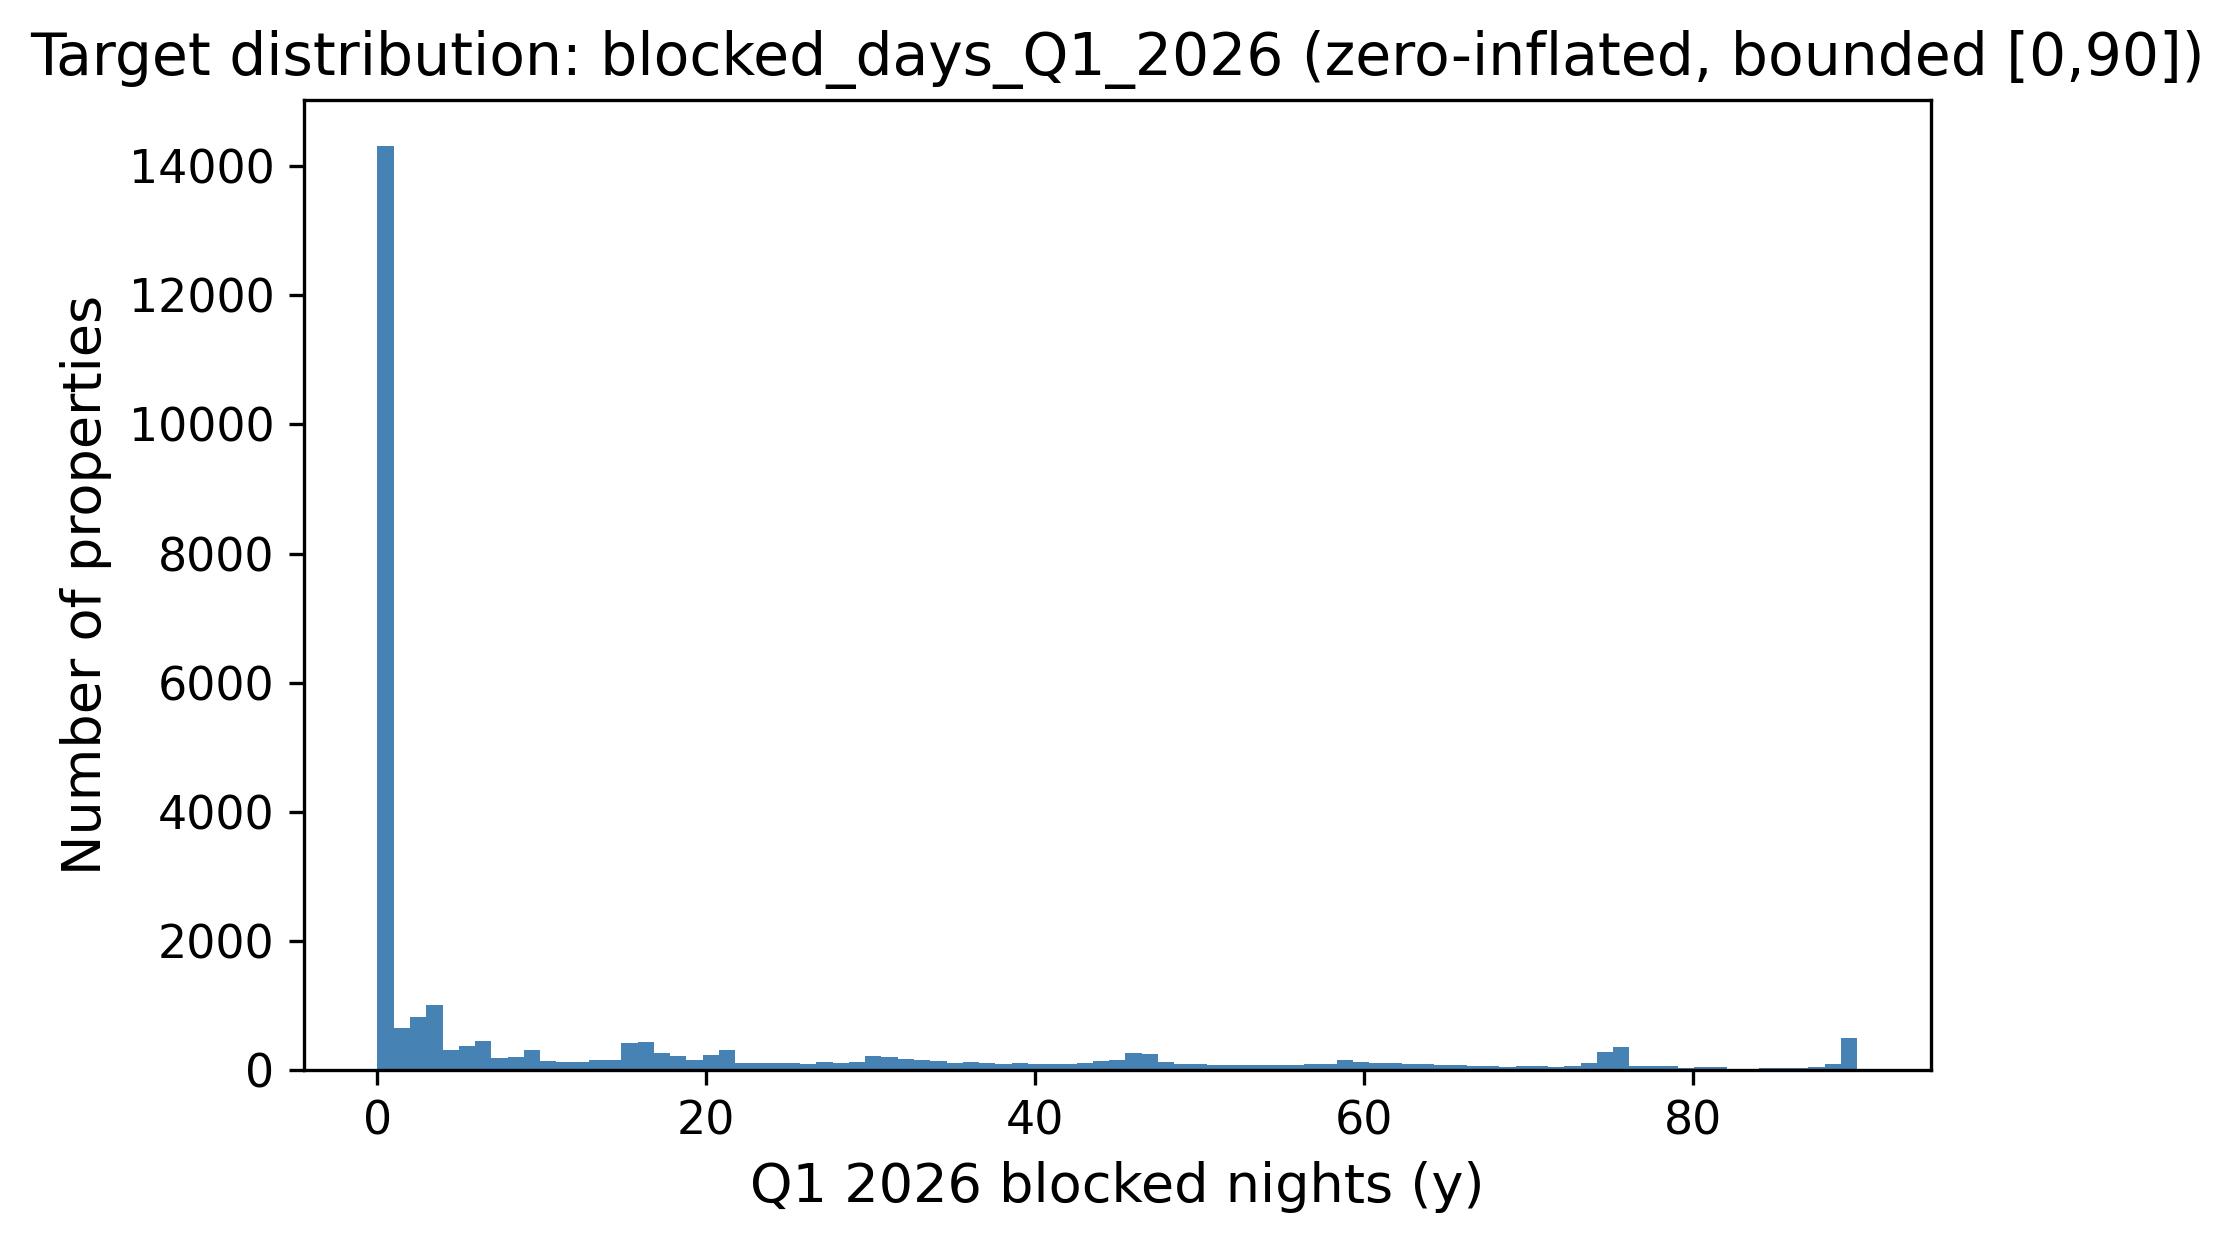
\includegraphics[width=\columnwidth]{fig1_target_dist.png}
\caption{Distribution of the target (Q1 2026 blocked nights, clean
multi-snapshot rule). The target is zero-inflated on the left and piles up
again near the 90-day maximum, which later justified clipping predictions to
$[0,90]$.}
\label{fig:target}
\end{figure}

Table~\ref{tab:targetstats} quantifies the shape of the clean target on the
full 36{,}261-listing universe. The mean (16.1) sits far above the median, the
distribution is strongly right-skewed (skewness $1.52$), and---most
importantly---49.6\% of properties were blocked for zero nights in Q1 2026,
while only 1.7\% reach the upper bound. This single statistic is what makes the
task a \emph{zero-inflated, bounded} regression problem rather than an ordinary
one, and it is the structural reason a least-squares estimator is biased at the
extremes (Sections~\ref{sec:linearcritique} and~\ref{sec:residuals}).
Table~\ref{tab:missing} lists the static columns with the highest missing
rates; because these are far from missing-at-random (a missing
\texttt{host\_response\_rate} typically marks an inactive host), we encode
missingness explicitly with indicator columns rather than discarding it.

\begin{table}[!t]
\caption{Target statistics on the full listing universe ($n=36{,}261$), clean
multi-snapshot rule.}
\label{tab:targetstats}
\centering
\begin{tabular}{lc}
\toprule
Statistic & Value \\
\midrule
Mean & 16.1 \\
Median & 1 \\
Standard deviation & 25.1 \\
Skewness & 1.52 \\
Rows with $y=0$ & 49.6\% \\
Rows with $y=90$ & 1.7\% \\
\bottomrule
\end{tabular}
\end{table}

\begin{table}[!t]
\caption{Missing-value rates of the most affected static columns.}
\label{tab:missing}
\centering
\begin{tabular}{lc}
\toprule
Column & Missing rate \\
\midrule
\texttt{price} (raw) & 100\% \\
\texttt{host\_response\_rate/time} & 41.8\% \\
\texttt{beds} & 41.1\% \\
\texttt{bathrooms} & 40.8\% \\
\texttt{review\_scores\_*} & 31.3\% \\
\bottomrule
\end{tabular}
\end{table}

\subsection{Feature Engineering}
\label{sec:featuregroups}
The core of the project was turning the listings snapshot and the six H2-2025
calendar/review histories into a single flat matrix with one row per listing
\texttt{id}, built \emph{strictly} from data through December 2025. We ended up
with 206 columns (205 numeric, 1 raw categorical). They fall into the following
groups.
\begin{itemize}
\item \textbf{Per-quarter calendar aggregates (Q3, Q4, and combined H2).} For
each listing we counted the days observed, blocked, and available, and derived
blocking/available rates, separately for Q3 2025 (Jul--Sep), Q4 2025 (Oct--Dec),
and the combined half year, so the model sees both levels and the Q3-to-Q4
trend.
\item \textbf{Monthly blocking rates and status transitions.} The blocking rate
in each of the six individual months, plus counts of available$\to$blocked and
blocked$\to$available transitions (\texttt{new\_blockings}/\texttt{new\_unblockings})
within Q3, Q4, and H2 --- a listing that changes state often is an active one.
\item \textbf{Recency and trajectory.} The same aggregates computed only over
the most recent observed window, plus a small least-squares trend
(\texttt{traj\_slope}, \texttt{traj\_accel}, recent-vs-older blocking-rate ratio)
fit over the last few weeks of H2, so an accelerating listing is distinguished
from one that is merely busy on average.
\item \textbf{Cross-snapshot calendar volatility.} Because Inside Airbnb
re-scrapes the same future dates every month, we can directly observe how often
a listing's recorded availability for a given date \emph{flips} between
consecutive H2-2025 scrapes (\texttt{h2\_flips}, \texttt{h2\_flip\_rate}) ---
this turned out to be the single strongest predictor in the whole matrix
(Fig.~\ref{fig:corr}) and has no analogue in the original 2016 data, which only
ever supplied one daily status per date.
\item \textbf{Price and revenue.} Price mean/min/max/range and the number of
distinct prices observed over the last five calendar snapshots, plus Airbnb's
own precomputed \texttt{estimated\_occupancy\_l365d} and
\texttt{estimated\_revenue\_l365d}, and a price-relative-to-neighbourhood
feature; because the raw \texttt{price} column in the listings table is 100\%
missing in this export, all price signal here is reconstructed from the daily
calendar price field.
\item \textbf{Reviews.} Review counts over 30/90/180/365-day windows and a
review-velocity acceleration term (90-day count vs.\ the preceding 90-day
count), plus the static review-score sub-ratings.
\item \textbf{Neighbourhood/geo context.} Leakage-safe context features ---
each listing's neighbourhood and K-Means geo-cluster ($k$-means on
latitude/longitude) mean blocking rate and density, computed only from the
purely historical \texttt{recent\_blocking\_rate} signal, plus the listing's own
rate relative to its neighbourhood/cluster.
\item \textbf{Property, host, and amenities.} Accommodates/bedrooms/bathrooms,
listing age, host tenure and listing-count fields, boolean host flags
(Superhost, instant-bookable), and 14 binary amenity flags (wifi, kitchen, air
conditioning, self check-in, long-term-stay friendly, etc.) parsed from the
JSON \texttt{amenities} column.
\item \textbf{Text keywords and property type.} Binary flags for words in the
listing title (``luxury,'' ``private,'' ``cozy,'' ``modern,'' ``view,'' etc.)
plus title length and word count, and one-hot room-/property-type groups.
\item \textbf{Raw categorical.} \texttt{neighbourhood\_cleansed} is kept as a
single raw high-cardinality categorical column rather than flattened at feature-
engineering time, and is one-hot- or target-encoded \emph{inside} each model's
own cross-validation fold (Section~\ref{sec:preproc}), matching how the
neighbourhood/borough categoricals were treated in the original 2016 pipeline.
\end{itemize}

Table~\ref{tab:featgroups} summarizes the families and their sizes. The
dominant families by count are the calendar aggregates, the geography/host
blocks, and the amenity/keyword flags, but the correlation analysis
(Fig.~\ref{fig:corr}) shows that raw count does not track predictive power: the
handful of cross-snapshot volatility and recency features outweigh the much
larger static-metadata block.

\begin{table}[!t]
\caption{Engineered feature families (206 columns total: 205 numeric,
1 raw categorical).}
\label{tab:featgroups}
\centering
\small
\begin{tabular}{lcp{1.15in}}
\toprule
Family & \# & Representative feature \\
\midrule
Geography (incl.\ geo-clusters) & 21 & latitude, geo\_cluster\_\{k\} \\
Host & 16 & host tenure, listing counts \\
Other property metadata & 16 & accommodates, bedrooms \\
Calendar H2 (combined) & 15 & \texttt{h2\_blocking\_rate} \\
Calendar Q3 & 14 & \texttt{q3\_blocking\_rate} \\
Amenities & 14 & \texttt{amen\_wifi}, \texttt{amen\_ac} \\
Recency window & 13 & \texttt{recent\_blocking\_rate} \\
Calendar Q4 & 12 & \texttt{q4\_blocking\_rate} \\
Text keywords & 10 & ``luxury''/``private'' flags \\
Price / revenue & 8 & \texttt{estimated\_revenue\_l365d} \\
Review scores & 8 & \texttt{review\_scores\_rating} \\
Trajectory & 7 & \texttt{traj\_slope}, \texttt{traj\_accel} \\
Property type & 7 & room-type one-hot \\
Calendar monthly & 6 & \texttt{m11\_blocking\_rate} \\
Nbhd/geo context & 6 & \texttt{nb\_mean\_rate}, \texttt{geo\_density} \\
Reviews (velocity) & 5 & \texttt{rev\_90d}, \texttt{rev\_accel\_90} \\
Borough & 5 & borough one-hot, freq.\ enc.\ \\
Cross-table ratios & 4 & \texttt{q3\_to\_q4\_blocking\_ratio} \\
Raw categorical & 1 & \texttt{neighbourhood\_cleansed} \\
\bottomrule
\end{tabular}
\end{table}

\begin{figure}[!t]
\centering
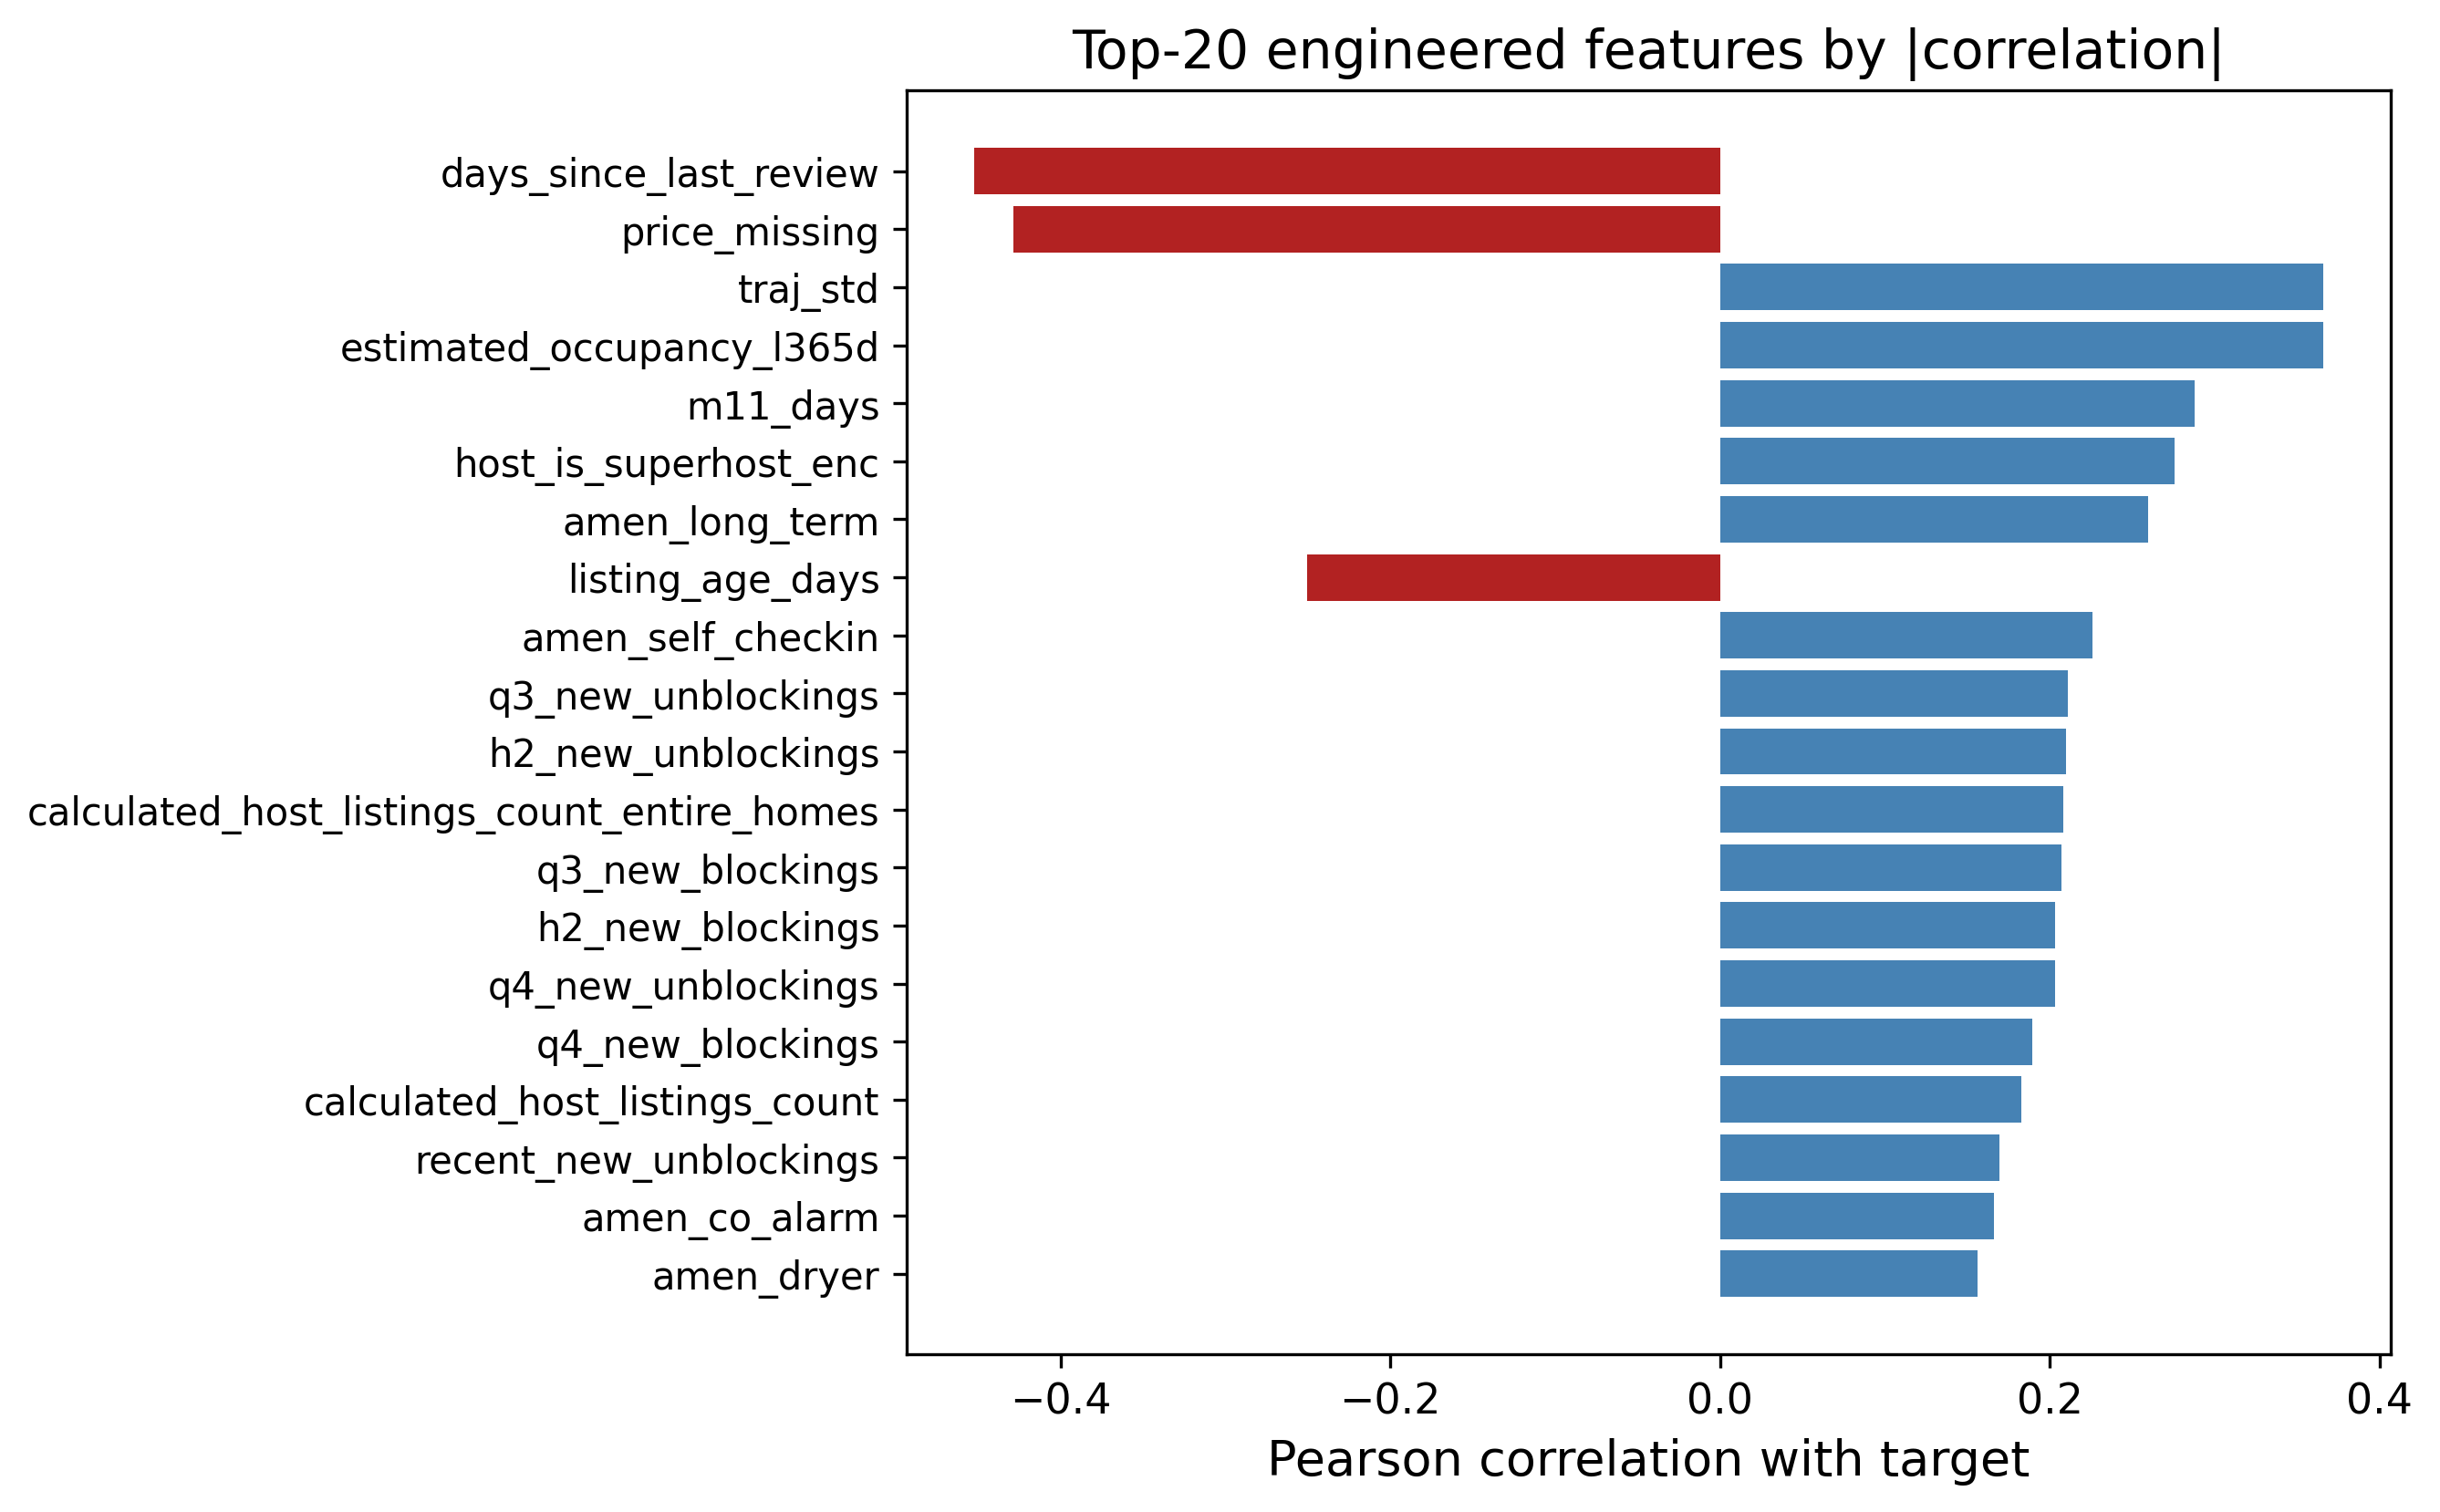
\includegraphics[width=\columnwidth]{fig2_top_corr.png}
\caption{Top engineered features by absolute correlation with the target. The
H2-2025 cross-snapshot calendar-volatility features (\texttt{h2\_flip\_rate},
\texttt{h2\_flips}) and recency/price signals dominate over static metadata.}
\label{fig:corr}
\end{figure}

\subsection{Preprocessing Pipeline and the Target Encoder}
\label{sec:preproc}
Every preprocessing step lives inside a scikit-learn \texttt{ColumnTransformer}
so that it is fit only on the training fold and then applied to the validation
fold, which keeps the workflow leakage-free. Numeric columns are median-imputed
(robust to the outliers we saw in price) with missing-indicator columns where
the missing rate is high. The one raw categorical column,
\texttt{neighbourhood\_cleansed}, is high-cardinality (well over 15 distinct
neighbourhoods), so we handle it two ways depending on the model: for Linear
Regression, Random Forest, and the MLP we cap it to its top-30 most frequent
levels (rarer levels collapse to \texttt{"Other"}) and one-hot encode; for the
gradient-boosted models (XGBoost, LightGBM, CatBoost) we instead use a custom
$K$-fold target encoder with additive smoothing, since trees benefit more from
a single smoothed numeric column than from 30 sparse binary ones.

\paragraph{Target-encoding formula} Let $y$ have global mean
$\mu=\tfrac{1}{n}\sum_{i=1}^{n}y_i$. For a categorical column, let level $c$
contain $n_c$ training rows with category mean
$\bar y_c=\tfrac{1}{n_c}\sum_{i:\,x_i=c}y_i$. The smoothed encoding for that
level is the count-weighted average of the category mean and the global prior,
\begin{equation}
e_c \;=\; \frac{n_c\,\bar y_c \;+\; \alpha\,\mu}{\,n_c+\alpha\,},
\qquad \alpha = 20,
\label{eq:smooth}
\end{equation}
where the smoothing factor $\alpha$ is, in effect, a number of ``pseudo-counts''
of the prior: when a level is rare ($n_c\!\ll\!\alpha$) the encoding shrinks
toward $\mu$, and when it is common ($n_c\!\gg\!\alpha$) it approaches the raw
category mean $\bar y_c$. Levels unseen at fit time map to $\mu$.

\paragraph{Leakage-free $K$-fold scheme} To prevent a row from informing its own
encoding, the encoder is fitted in an internal $K$-fold loop ($K=5$). Writing
$\mathcal{F}_1,\dots,\mathcal{F}_K$ for the inner folds, the encoded value of a
training row $i\in\mathcal{F}_k$ uses statistics computed \emph{only} on the
complementary folds,
\begin{equation}
\tilde e_i \;=\; e^{\,(-\mathcal{F}_k)}_{\,x_i},
\qquad i\in\mathcal{F}_k,
\label{eq:kfoldte}
\end{equation}
where $e^{\,(-\mathcal{F}_k)}_{c}$ is \eqref{eq:smooth} evaluated on
$\{(\mathbf{x}_j,y_j):j\notin\mathcal{F}_k\}$. At transform time (validation and
test rows) we use the full-data map.

To make \eqref{eq:smooth} concrete, consider a neighbourhood that appears in
$n_c=4$ training rows with a local mean of $\bar y_c=40$ blocked nights, against a
global mean of $\mu=16.1$. With $\alpha=20$ the encoded value is
$e_c=\frac{4\cdot 40+20\cdot 16.1}{4+20}=\frac{160+322}{24}\approx 20.1$, i.e.\
the estimate is pulled strongly back toward the global prior because only four
listings support it. A neighbourhood with $n_c=400$ rows and the same local mean
would instead encode to $\frac{400\cdot40+20\cdot16.1}{420}\approx 38.9$, almost
the raw mean. This shrinkage is precisely what stops rare high-cardinality levels
from injecting noisy, over-confident estimates into the model. For XGBoost we additionally lean on its
native missing-value handling rather than imputing, since it learns the best
split direction for NaNs on its own \cite{chen2016xgboost}. For the linear
baseline we apply \texttt{StandardScaler}; for the tree models scaling is
unnecessary, but we keep the rest of the pipeline identical so the comparison is
fair.

\subsection{Model Selection and Rationale}
We compare nine model configurations from four families and blend across all of
them.

\subsubsection{Linear Regression (baseline)}
A plain linear regression gives us an interpretable lower bar and tells us which
features are linearly related to the target; its structural limitation on this
bounded target is analysed in Section~\ref{sec:linearcritique}.

\subsubsection{Random Forest Regressor}
A bagging ensemble \cite{breiman1996,breiman2001} that is robust to noise and
needs little tuning. We use it as a strong non-linear reference point.

\subsubsection{Gradient Boosting, XGBoost, LightGBM, and CatBoost}
Boosting builds the model sequentially and is widely regarded as the best
off-the-shelf method for tabular data \cite{friedman2001,chen2016xgboost}. We
train a plain scikit-learn \texttt{GradientBoostingRegressor} as a weak
boosting reference, three XGBoost configurations (a hardcoded-parameter
``main'' model carried over from earlier exploration, and two independently
retuned variants, v2 and v3, described in Section~\ref{sec:tuning}), and two
additional modern boosting libraries, LightGBM \cite{ke2017lightgbm} and
CatBoost \cite{prokhorenkova2018catboost}, as further diverse ensemble members
for the blend. All of the XGBoost variants minimize the regularized objective
\begin{equation}
\mathcal{L}(\phi)=\sum_{i=1}^{n}\ell\!\big(y_i,\hat y_i\big)
+\sum_{t}\Omega(f_t),\quad
\Omega(f)=\gamma T+\tfrac{1}{2}\lambda\lVert\mathbf{w}\rVert^{2}
+\alpha\lVert\mathbf{w}\rVert_{1},
\label{eq:xgbobj}
\end{equation}
with squared-error loss $\ell(y,\hat y)=(y-\hat y)^2$, $T$ the number of leaves,
$\mathbf{w}$ the leaf weights, and $\gamma,\lambda,\alpha$ the complexity,
$L_2$, and $L_1$ penalties. LightGBM and CatBoost optimize the same squared-error
objective with their own leaf-growth strategies (leaf-wise for LightGBM,
symmetric/oblivious trees for CatBoost); we tune both with the same
fold-level-early-stopping search described in Section~\ref{sec:tuning}.

\subsubsection{Multi-Layer Perceptron (MLP)}
\label{sec:mlp}
Finally, we trained a small feed-forward neural network in PyTorch
\cite{paszke2019pytorch} with the Adam optimizer \cite{kingma2015adam}.
The network maps the preprocessed input
$\mathbf{z}^{(0)}=\mathbf{x}\in\mathbb{R}^{d}$ through three hidden blocks of
width $(h_1,h_2,h_3)=(256,128,64)$. Each block applies an affine map, batch
normalization, a ReLU non-linearity, and dropout with rate $p=0.2$:
\begin{align}
\mathbf{a}^{(\ell)} &= \mathbf{W}^{(\ell)}\mathbf{z}^{(\ell-1)}+\mathbf{b}^{(\ell)},
\label{eq:mlp_aff}\\
\mathbf{z}^{(\ell)} &= \mathrm{Dropout}_{p}\!\Big(\mathrm{ReLU}\big(
\mathrm{BN}(\mathbf{a}^{(\ell)})\big)\Big),\quad \ell=1,2,3,
\label{eq:mlp_block}
\end{align}
where $\mathrm{ReLU}(u)=\max(0,u)$ and batch normalization standardizes each
unit over the mini-batch $\mathcal{B}$,
\begin{equation}
\mathrm{BN}(a)=\gamma\,\frac{a-\mu_{\mathcal{B}}}{\sqrt{\sigma_{\mathcal{B}}^{2}+\epsilon}}+\beta .
\label{eq:bn}
\end{equation}
A linear read-out produces the scalar prediction in log space,
$\hat r=\mathbf{w}^{(4)\top}\mathbf{z}^{(3)}+b^{(4)}$. Because the count is
skewed, the network is trained on the log-transformed target
$t=\log(1+y)$ with the mean-squared-error criterion
$\mathcal{L}=\tfrac{1}{|\mathcal{B}|}\sum_{i\in\mathcal{B}}(\hat r_i-t_i)^2$, and
predictions are mapped back and clipped,
$\hat y=\mathrm{clip}\big(e^{\hat r}-1,\,0,\,90\big)$. Parameters are updated by
Adam with learning rate $\eta=10^{-3}$ and $L_2$ weight decay $10^{-5}$; using
the standard moment estimates $\mathbf{m}_t,\mathbf{v}_t$ of the gradient
$\mathbf{g}_t$,
\begin{equation}
\boldsymbol{\theta}_{t+1}=\boldsymbol{\theta}_{t}
-\eta\,\frac{\hat{\mathbf m}_t}{\sqrt{\hat{\mathbf v}_t}+\epsilon},
\quad
\hat{\mathbf m}_t=\frac{\mathbf m_t}{1-\beta_1^{t}},\;
\hat{\mathbf v}_t=\frac{\mathbf v_t}{1-\beta_2^{t}}.
\label{eq:adam}
\end{equation}
Training uses a batch size of 512 for up to 60 epochs with early stopping on a
held-out validation MSE (patience 8). Going in, the literature
\cite{tang2024,camatti2024} led us to expect the trees to win, and they
did---but the MLP turned out to be a useful blend partner because its errors
were not perfectly correlated with the trees' (Section~\ref{sec:complementarity}).

A few design choices deserve a note. Unlike the final XGBoost, the MLP is
trained on the log-transformed target $\log(1+y)$ rather than the raw count.
Neural networks are sensitive to the scale and skew of the target, and the raw
target's long right tail produced unstable gradients and slow convergence; the
log transform compresses that tail so the squared-error loss is better
conditioned, and the monotone inverse $e^{\hat r}-1$ followed by clipping returns
predictions to the count scale. This is not a contradiction with our decision to
\emph{drop} the log transform for XGBoost (Section~\ref{sec:changes}): boosted
trees are invariant to monotone feature scaling and optimize the raw-scale loss
directly, so for them the transform only distorted the objective, whereas for the
MLP it is a numerical-stability aid. Batch normalization
\eqref{eq:bn} keeps the pre-activations well scaled across the three hidden
layers, and dropout ($p=0.2$) plus the $L_2$ weight decay in \eqref{eq:adam}
regularize a network that would otherwise overfit a 29{,}008-row table with 206
inputs.

\subsection{Hyper-Parameter Tuning}
\label{sec:tuning}
All tuning is done with 5-fold cross-validation on the 80\% development split.
For XGBoost we wrote our own randomized search instead of using
\texttt{RandomizedSearchCV}, because we wanted fold-level early stopping: inside
each of the five outer folds we carve out a small internal validation set, fit
up to $B_{\max}=3000$ trees with \texttt{early\_stopping\_rounds}~$=50$, and keep
only the best iteration. \texttt{RandomizedSearchCV} does not let us pass a
per-fold \texttt{eval\_set} cleanly, so a custom loop was the simplest correct
option, and it also let us log every configuration we tried.

\paragraph{Search objective} Let $\Theta$ be the hyper-parameter space and let
the data be partitioned into outer folds $\mathcal{D}_1,\dots,\mathcal{D}_K$
($K=5$). For a configuration $\theta$, within fold $k$ we split the training part
into a fitting set and an inner validation set $\mathcal{V}_k$, grow boosting
iterations $b=1,\dots,B_{\max}$, and select the early-stopping iteration
\begin{equation}
b_k^{*}(\theta)=\operatorname*{arg\,min}_{1\le b\le B_{\max}}
\;\mathrm{RMSE}\!\Big(y^{\mathcal{V}_k},\,
\hat f^{(b)}_{\theta,k}\big(\mathbf{X}^{\mathcal{V}_k}\big)\Big),
\label{eq:earlystop}
\end{equation}
stopping once no improvement is seen for 50 consecutive rounds. The search then
minimizes the mean cross-validated MSE of the early-stopped models,
\begin{equation}
\theta^{*}=\operatorname*{arg\,min}_{\theta\in\Theta}\;
\frac{1}{K}\sum_{k=1}^{K}
\mathrm{MSE}\!\Big(y^{\mathcal{D}_k},\,
\hat f^{\,(b_k^{*}(\theta))}_{\theta,k}\big(\mathbf{X}^{\mathcal{D}_k}\big)\Big).
\label{eq:searchobj}
\end{equation}
We ran this search twice for independent XGBoost variants, drawing $N=30$
configurations for ``v2'' and $N=60$ for ``v3,'' both from the product of the
marginals in Table~\ref{tab:search}, sampling the learning rate and the
regularization terms log-uniformly so that small and large scales are explored
evenly, as recommended by \cite{bergstra2012random}. The full procedure is
summarized in Algorithm~1. LightGBM and CatBoost are tuned with the same
fold-level-early-stopping principle over $N=40$ draws each, but over their own
native parameter spaces (\texttt{num\_leaves}, \texttt{min\_child\_samples} for
LightGBM; \texttt{depth}, \texttt{l2\_leaf\_reg} for CatBoost). The ``main''
XGBoost configuration (used in the baseline comparison of
Table~\ref{tab:cv}) instead carries fixed, hand-set hyper-parameters from
earlier exploratory runs, with no independent search or early stopping of its
own in this iteration of the pipeline; comparing its score to the
independently-tuned v2/v3 variants (Table~\ref{tab:metrics}) is itself an
informal check on how much headroom the search actually finds.

\begin{table}[!t]
\caption{Search distributions for the randomized search (used for both the v2
and v3 XGBoost variants). $\mathrm{LogU}$ denotes a log-uniform draw,
$\mathcal{U}$ a uniform draw.}
\label{tab:search}
\centering
\begin{tabular}{ll}
\toprule
Hyper-parameter & Sampling distribution \\
\midrule
\texttt{n\_estimators} (cap $B_{\max}$) & $3000$ (fixed) \\
\texttt{learning\_rate} & $\mathrm{LogU}(0.02,\,0.10)$ \\
\texttt{max\_depth} & $\mathcal{U}\{4,\dots,8\}$ \\
\texttt{min\_child\_weight} & $\mathcal{U}\{1,\dots,11\}$ \\
\texttt{subsample} & $\mathcal{U}(0.65,\,0.95)$ \\
\texttt{colsample\_bytree} & $\mathcal{U}(0.65,\,0.95)$ \\
\texttt{gamma} ($\gamma$) & $\mathcal{U}(0.0,\,0.4)$ \\
\texttt{reg\_alpha} ($\alpha$) & $\mathrm{LogU}(10^{-3},\,0.5)$ \\
\texttt{reg\_lambda} ($\lambda$) & $\mathrm{LogU}(0.5,\,5.0)$ \\
\bottomrule
\end{tabular}
\end{table}

\vspace{2pt}
\noindent\textbf{Algorithm 1: Randomized search with fold-level early stopping.}
\emph{Input:} hyper-parameter space $\Theta$, outer folds
$\{\mathcal{D}_k\}_{k=1}^{K}$, budget $N$, tree cap $B_{\max}$.
\begin{enumerate}
\item Initialize $\theta^{*}\leftarrow\varnothing$, $s^{*}\leftarrow+\infty$.
\item For $j=1,\dots,N$: sample a configuration $\theta\sim\Theta$ from
Table~\ref{tab:search}.
\item For each fold $k=1,\dots,K$: fit the preprocessing on the training part,
carve an inner validation set $\mathcal{V}_k$, grow up to $B_{\max}$ trees, pick
the early-stop iteration $b_k^{*}$ by \eqref{eq:earlystop}, and record
$m_k=\mathrm{MSE}$ on $\mathcal{D}_k$ using $b_k^{*}$ trees.
\item Set $s=\frac{1}{K}\sum_k m_k$ and log $(\theta,s)$; if $s<s^{*}$, update
$s^{*}\leftarrow s$, $\theta^{*}\leftarrow\theta$.
\item After $N$ configurations, return $\theta^{*}$.
\end{enumerate}
\vspace{2pt}

Our best v3 configuration (Table~\ref{tab:xgbparams}) used a learning rate of
0.026, max depth 8, subsample 0.80, and \texttt{colsample\_bytree} 0.68, and
early stopping settled around 363 trees on average -- despite a search cap of
3{,}000, none of the 60 configurations needed anywhere near that many
iterations before its held-out validation error stopped improving. The v2
search (30 configurations) converged to an almost identical region (learning
rate 0.025, max depth 8, $\approx$363 trees) and a nearly identical score
(Table~\ref{tab:metrics}), which is a useful sanity check: two independent
searches over the same space landed in the same neighbourhood rather than at
different local optima.

\begin{table}[!t]
\caption{Best XGBoost (v3) hyper-parameters found by the 60-configuration
randomized search.}
\label{tab:xgbparams}
\centering
\begin{tabular}{ll}
\toprule
Hyper-parameter & Value \\
\midrule
\texttt{n\_estimators} (cap) & 3000 \\
\texttt{learning\_rate} & 0.0262 \\
\texttt{max\_depth} & 8 \\
\texttt{min\_child\_weight} & 3 \\
\texttt{subsample} & 0.804 \\
\texttt{colsample\_bytree} & 0.680 \\
\texttt{gamma} & 0.314 \\
\texttt{reg\_alpha} & 0.0158 \\
\texttt{reg\_lambda} & 3.244 \\
\texttt{early\_stopping\_rounds} & 50 ($\approx$363 trees kept) \\
\bottomrule
\end{tabular}
\end{table}

\noindent\emph{Note.} The independently-tuned search (295.8 CV MSE for v3,
Table~\ref{tab:metrics}) essentially matched, rather than clearly beat, the
hand-set ``main'' XGBoost configuration (295.7 CV MSE) that we carried over
from earlier exploration without a dedicated search of its own. We view this as
an honest, informative negative result rather than a wasted search: on this
feature set, a reasonably-chosen manual configuration and a 30--60 iteration
randomized search reach comparable error, which suggests that on this problem
the ceiling is set more by the feature matrix than by exact tree
hyper-parameters (Section~\ref{sec:ablation}).

\subsection{Ensembling (Weighted Blend)}
\label{sec:blend}
Rather than submit a single model, we combine the out-of-fold (OOF) predictions
of the candidate models with a convex weighted average. Stack the $m$ models'
OOF predictions into a matrix $\mathbf{P}\in\mathbb{R}^{n\times m}$ with column
$j$ holding model $j$'s OOF prediction. We seek weights
$\mathbf{w}\in\mathbb{R}^{m}$ that minimize the blended MSE, subject to the
predictions staying on the valid scale:
\begin{align}
\min_{\mathbf{w}\in\mathbb{R}^{m}}\quad
& \frac{1}{n}\sum_{i=1}^{n}\Big(y_i-\mathrm{clip}\big[(\mathbf{P}\mathbf{w})_i,\,0,\,90\big]\Big)^{2}
\label{eq:blendobj}\\
\text{s.t.}\quad & \sum_{j=1}^{m}w_j = 1,
\label{eq:blendeq}\\
& 0 \le w_j \le 1,\quad j=1,\dots,m.
\label{eq:blendbox}
\end{align}
The equality constraint~\eqref{eq:blendeq} and the box
bounds~\eqref{eq:blendbox} make the solution a \emph{convex combination}, which
keeps the blend on the same scale as the inputs and prevents any single model
from receiving a runaway weight. We solve \eqref{eq:blendobj}--\eqref{eq:blendbox}
with Sequential Least-Squares Quadratic Programming (SLSQP) via
\texttt{scipy.optimize.minimize}, starting from the uniform point
$w_j^{(0)}=1/m$ with \texttt{ftol}~$=10^{-9}$. As a post-processing step we zero
out negligible weights ($w_j<10^{-4}$) and renormalize so that
\eqref{eq:blendeq} still holds exactly. We also ran a randomized search directly
over the weight simplex as a sanity check and obtained the same optimum, which
confirms the SLSQP solution is not an artefact of that particular optimizer.
Across the nine candidate models, the optimizer concentrated most of the weight
on the main XGBoost ($\approx0.45$), with substantial secondary weight on
LightGBM ($\approx0.18$) and Random Forest ($\approx0.16$), smaller
contributions from XGBoost v3 ($\approx0.10$), CatBoost ($\approx0.07$), and the
MLP ($\approx0.05$), a negligible weight on XGBoost v2 ($\approx0.004$), and
Linear Regression and the plain Gradient Boosting baseline dropped to zero
(Table~\ref{tab:weights}). The full procedure is given in Algorithm~2.

\vspace{2pt}
\noindent\textbf{Algorithm 2: Convex weighted blend via SLSQP.}
\emph{Input:} OOF matrix $\mathbf{P}\in\mathbb{R}^{n\times m}$, targets
$\mathbf{y}$.
\begin{enumerate}
\item Define the objective
$g(\mathbf{w})=\frac{1}{n}\lVert\mathbf{y}-\mathrm{clip}(\mathbf{P}\mathbf{w},0,90)\rVert_2^2$.
\item Initialize $\mathbf{w}^{(0)}=(1/m,\dots,1/m)$.
\item Minimize $g$ with SLSQP subject to $\sum_j w_j=1$ and $0\le w_j\le1$ to
obtain $\mathbf{w}^{*}$.
\item Prune: set $w_j^{*}=0$ for every $j$ with $w_j^{*}<10^{-4}$.
\item Renormalize $\mathbf{w}^{*}\leftarrow\mathbf{w}^{*}/\sum_j w_j^{*}$ and
return $\mathbf{w}^{*}$.
\end{enumerate}
\vspace{2pt}

\subsection{Experimental Design and Evaluation}
We split the labelled data once into an 80\% development set (29{,}008
properties) and a 20\% local hold-out (7{,}253 properties) with a fixed seed, so
every model is trained and selected on exactly the same rows, and the hold-out
is touched only for the final numbers reported in
Section~\ref{sec:results}. Inside the development set we use 5-fold
cross-validation for both model selection and tuning. We optimise MSE directly,
but we also track MAE and $R^2$ internally because they are easier to read. To
stop leakage, we (i) fit every preprocessing step only on the training fold,
(ii) build no feature from any 2026 information (Section~\ref{sec:dataset}),
and (iii) compute target encodings inside their own inner $K$-fold per
\eqref{eq:kfoldte}. As a last step we clip predictions to $[0,90]$, both
because no property can be blocked more than 90 nights in a 90-day quarter and
to bound the loss contributed by any stray extrapolation.

\subsection{Computational Cost}
\label{sec:cost}
Because the project ran on a single workstation rather than a cluster, we kept
an eye on cost throughout. Building the 206-feature matrix from the 79 million
H2-2025 calendar/review rows is a one-time aggregation that dominates
wall-clock time but is trivially parallelizable over listings. Model training
is cheap by comparison: a single early-stopped XGBoost fit converges at
$\approx$363 trees on average, so the 60-configuration v3 randomized search
(Algorithm~1) and the 30-configuration v2 search each complete in well under
an hour on commodity hardware. The Random Forest, LightGBM, and CatBoost
searches are of the same order; the linear, MLP, and plain gradient-boosting
baselines are faster still. The SLSQP blend itself is essentially
free---it optimizes only $m=9$ weights over a fixed $n\times m$ matrix of
cached OOF predictions, converging in well under a second. This favourable cost
profile is one practical reason we preferred a small, well-tuned ensemble over a
single very large model: the marginal compute of adding the blend is negligible
relative to the searches, yet it returns a statistically significant accuracy
gain (Section~\ref{sec:significance}).

\subsection{Reproducibility and Implementation}
\label{sec:repro}
Every result in this paper is reproducible from a single fixed seed
(\texttt{random\_state}~$=42$), which governs the 80/20 development/hold-out
split, the 5-fold cross-validation partitions, the inner target-encoding folds,
and the random-search samplers. The pipeline is implemented entirely in Python
with scikit-learn \cite{pedregosa2011sklearn} for the preprocessing
\texttt{ColumnTransformer}, imputers, one-hot encoder, linear, random-forest and
gradient-boosting models and cross-validation; the \texttt{xgboost}
\cite{chen2016xgboost}, \texttt{lightgbm} \cite{ke2017lightgbm}, and
\texttt{catboost} \cite{prokhorenkova2018catboost} packages for the boosted
trees; PyTorch \cite{paszke2019pytorch} with Adam \cite{kingma2015adam} for the
MLP; and \texttt{scipy.optimize} for the SLSQP blend. The code is organized as
a sequence of 15 numbered notebooks---exploratory analysis, feature
engineering, one notebook per model family (including three XGBoost variants
and a dedicated hurdle-model notebook), the blend, an incremental ablation, and
a figures notebook---so that each stage can be re-run independently, and the
out-of-fold predictions are cached to disk (\texttt{.npy}) so that the blend
and all of the post-hoc diagnostics in Section~\ref{sec:results} can be
recomputed without retraining.

%==============================================================================
\section{Results and Discussion}
\label{sec:results}
Table~\ref{tab:cv} lists the 5-fold cross-validation scores of all nine model
configurations on the development set. The ordering is exactly what the
literature predicted. Linear Regression and the plain (untuned)
\texttt{GradientBoostingRegressor} trailed the field, Random Forest and the MLP
sat in the middle, and the boosted-tree family (XGBoost and its variants,
LightGBM, CatBoost) clustered tightly together at the top, all within about 2
MSE points of one another. The hand-set main XGBoost configuration (295.7) and
the independently 60-configuration-tuned XGBoost v3 (295.8) are statistically
indistinguishable, and the SLSQP blend of all nine models pushed the
out-of-fold error down to 290.1 --- about a 1.9\% relative improvement over the
best single model, consistent with the modest but real gains typically reported
for blending closely-correlated tree ensembles.

\begin{table}[!t]
\caption{5-fold CV results on the development set, all nine model
configurations (lower MSE is better).}
\label{tab:cv}
\centering
\begin{tabular}{lccc}
\toprule
Model & MSE & MAE & $R^2$ \\
\midrule
XGBoost (main) & 295.7 & 10.05 & 0.531 \\
XGBoost v3 (retuned) & 295.8 & --- & --- \\
LightGBM (retuned) & 296.5 & 10.20 & 0.529 \\
XGBoost v2 (retuned) & 296.9 & --- & --- \\
CatBoost (retuned) & 301.5 & 10.43 & 0.522 \\
RandomForest & 302.8 & 10.32 & 0.519 \\
LinearRegression & 357.6 & 12.24 & 0.432 \\
MLP & 382.5 & 10.40 & 0.393 \\
GradientBoosting & 435.8 & 11.04 & 0.308 \\
\midrule
\textbf{SLSQP blend (9 models)} & \textbf{290.1} & \textbf{10.02} & \textbf{0.540} \\
\bottomrule
\end{tabular}
\end{table}

\begin{figure}[!t]
\centering
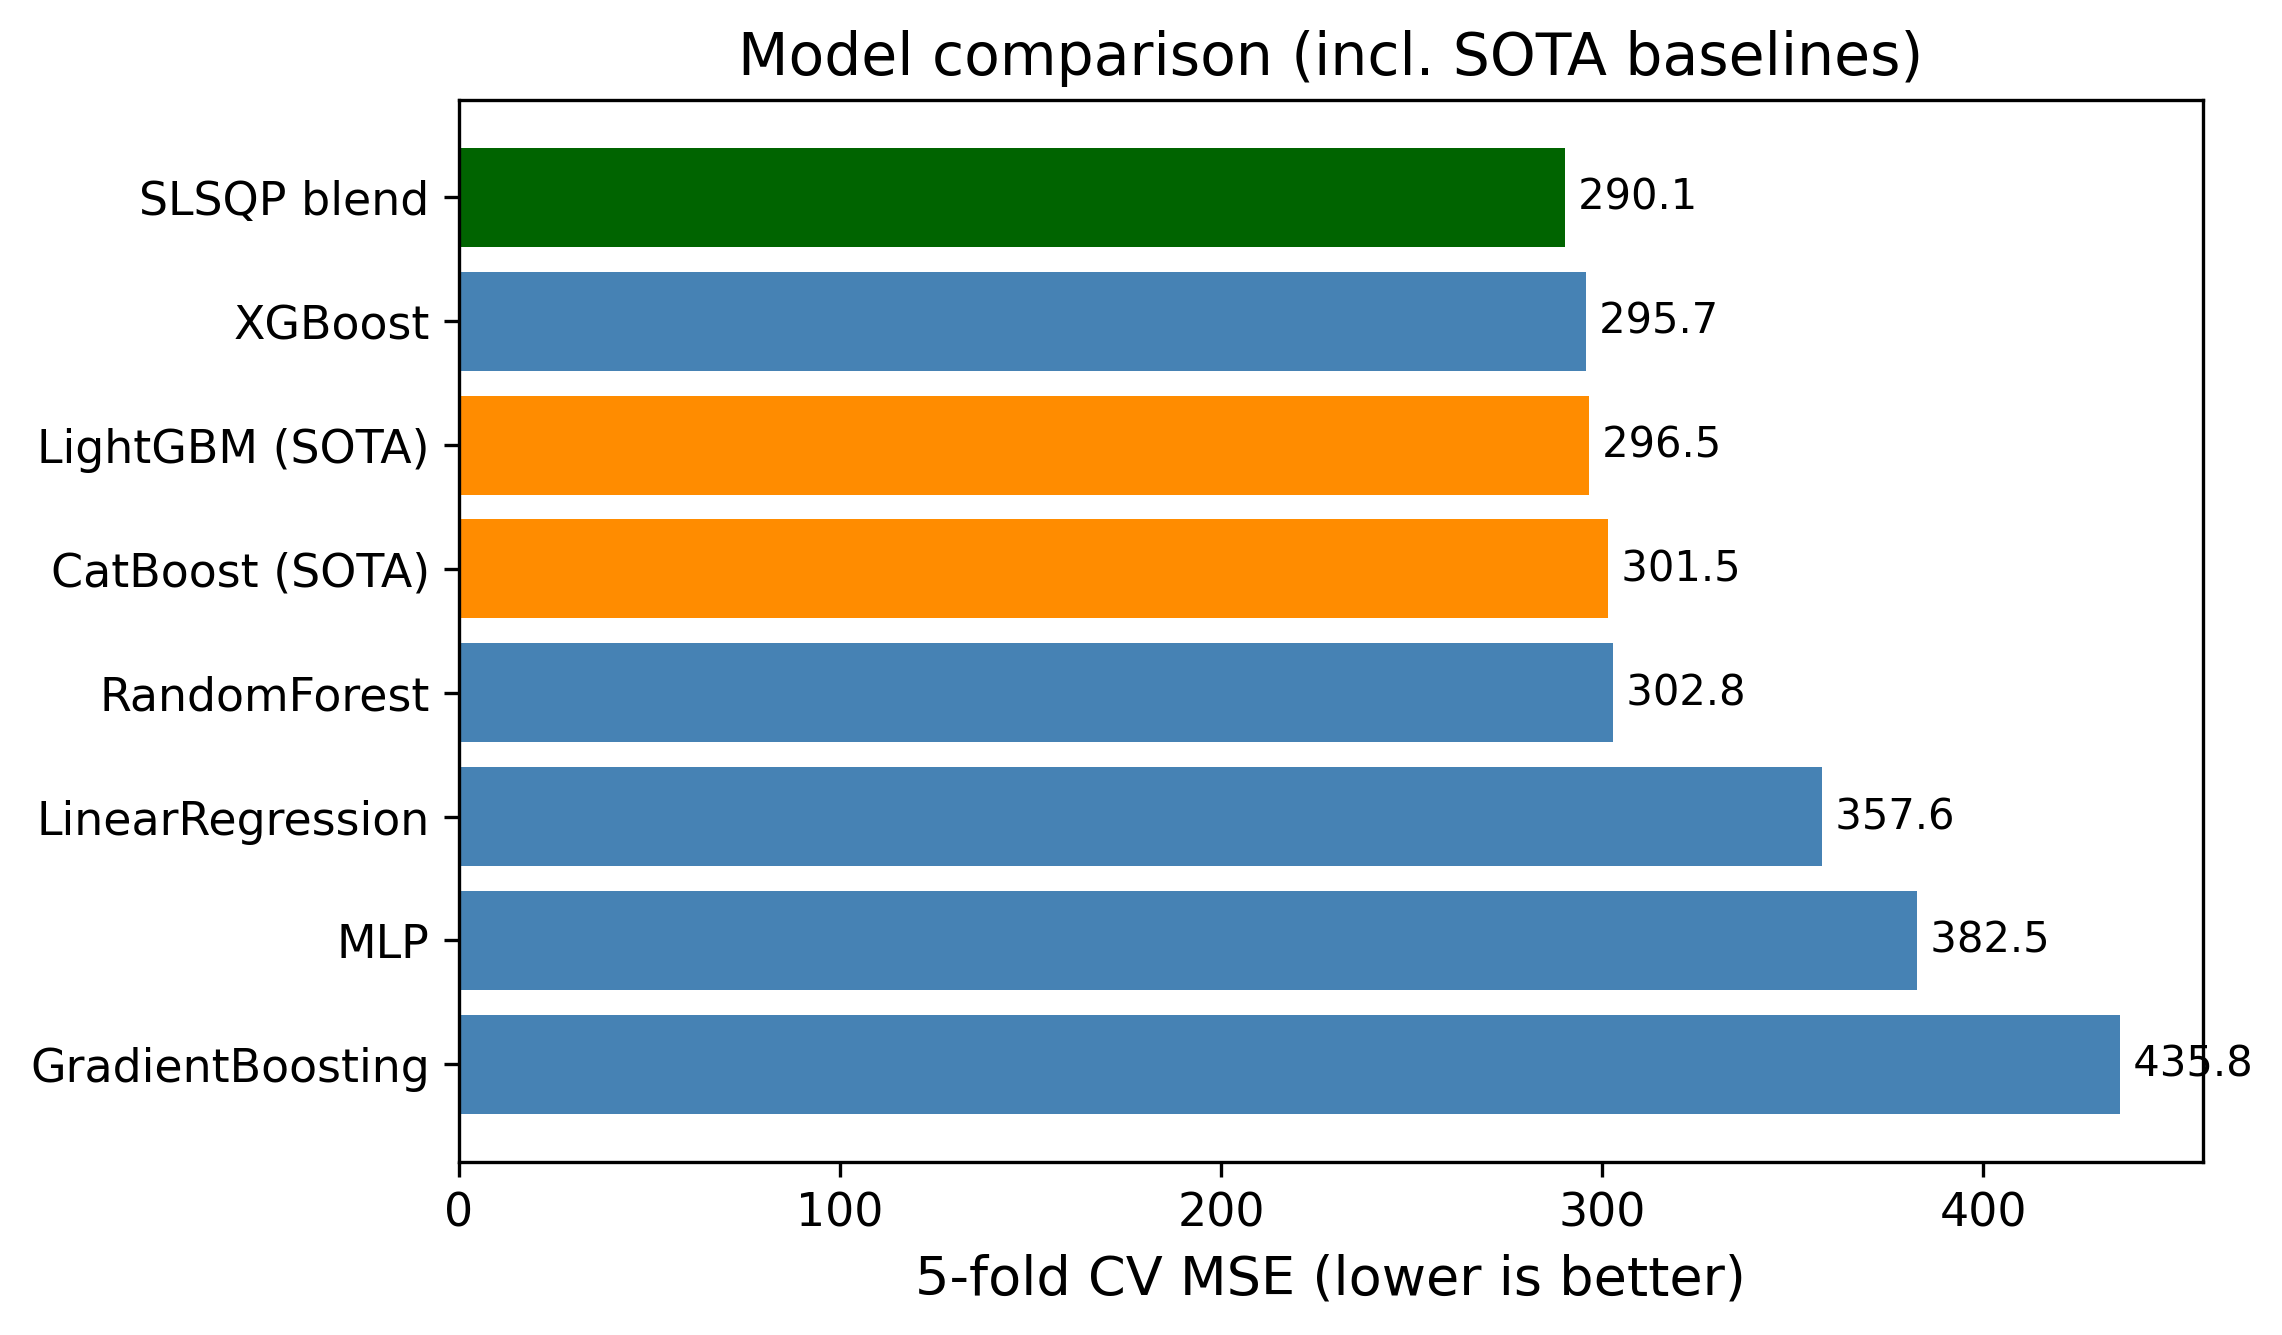
\includegraphics[width=\columnwidth]{fig3_baseline_cv.png}
\caption{Model comparison by cross-validated MSE, including the LightGBM/
CatBoost baselines and the final blend. The tree-based models cluster tightly
at the top; Linear Regression, the MLP, and the untuned Gradient Boosting
trail well behind.}
\label{fig:baseline}
\end{figure}

\subsection{Incremental Ablation}
\label{sec:ablation}
To make the source of the final error reduction explicit rather than implicit
in the model comparison above, we ran a single incremental ablation, adding one
change at a time on top of a Linear Regression baseline and reporting 5-fold CV
MSE after each step (Table~\ref{tab:ablation}). Starting from the 15 raw static
listing columns alone (384.4 MSE), adding the full 206-column engineered
feature matrix (still with the raw categorical dropped rather than encoded)
brings the largest single drop of the whole ablation (-24.2, to 360.2) --
feature engineering, not modelling, is where most of the ceiling is set on this
problem, echoing the point made in Section~\ref{sec:lit}. Adding the $K$-fold
target encoding of \texttt{neighbourhood\_cleansed} on top of that is
essentially free (-0.1): on this dataset the raw categorical carries very
little signal beyond what the calendar/recency features already capture, unlike
in the original 2016 dataset where neighbourhood carried more independent
price information. Switching from a linear model to a tuned XGBoost on the same
full feature matrix is the second-largest drop (-64.3, to 295.7), confirming
the non-linearity argument of Section~\ref{sec:linearcritique} empirically. An
\emph{equal}-weight blend of all nine models is actually a step backwards
(+5.2, to 301.0), since it lets the weak learners drag the average down; only
once the weights are chosen by SLSQP does blending help (-10.8, to 290.1). The
overall picture is that feature engineering and the switch to tree ensembles
each mattered far more than target encoding or than na\"ive blending, and only
a properly \emph{weighted} blend recovers a genuine, if small, additional gain.

\begin{table}[!t]
\caption{Incremental ablation (5-fold CV MSE, $\mathtt{random\_state}=42$).}
\label{tab:ablation}
\centering
\small
\begin{tabular}{lcc}
\toprule
Configuration & MSE & $\Delta$ \\
\midrule
Linear Reg., raw static features only & 384.4 & --- \\
\quad + 206 engineered features (no TE) & 360.2 & $-24.2$ \\
\quad + $K$-fold target encoding (full prep.) & 360.0 & $-0.1$ \\
XGBoost (tuned, full preprocessing) & 295.7 & $-64.3$ \\
\quad Equal-weight blend of 9 learners & 301.0 & $+5.2$ \\
\quad SLSQP convex blend & 290.1 & $-10.8$ \\
\bottomrule
\end{tabular}
\end{table}

\subsection{Why the Methods Behaved as They Did}
The gap between the linear model and the boosted trees is the clearest result,
and it is exactly the structural mismatch we made precise in
Section~\ref{sec:linearcritique}: the relationship between our features and the
bounded, zero-inflated target is strongly non-linear and full of
interactions---for example, a high H2-2025 blocking rate means something very
different for a listing whose calendar has been flipping back and forth every
month than for one that has been stably booked. Linear regression cannot
represent those interactions without hand-crafting them, while trees discover
them automatically. Random Forest captures the non-linearity but, being a
variance-reduction (bagging) method, it cannot reduce bias as aggressively as
boosting can. The boosted-tree family (XGBoost, LightGBM, CatBoost) combines low
bias (sequential residual fitting) with strong regularization and, for the v2/v3
XGBoost variants and the LightGBM/CatBoost search, early stopping, which is why
that whole family clusters at the top. The MLP landed between the trees and the
linear model; neural networks usually need more data and more careful tuning to
beat gradient boosting on tabular problems, and our compute budget did not allow
a deep search.

It is useful to read the whole ranking through a bias--variance lens. Linear
regression is a high-bias, low-variance estimator: it cannot bend to the
saturating conditional mean of Section~\ref{sec:linearcritique}, so its error is
dominated by bias and no amount of data removes it. Random Forest attacks the
opposite term---bagging averages many high-variance trees to cut variance---but,
because every tree is grown to near-purity on the same features, it leaves a
residual bias that boosting can still reduce. Gradient boosting lowers bias by
fitting residuals stage by stage, and the tuned boosted-tree models add the
regularization and early stopping \eqref{eq:xgbobj}--\eqref{eq:earlystop} that
keep the corresponding variance in check, which is why they sit at the bottom
of the MSE column. The MLP is capable of low bias in principle, but on
29{,}008 rows it is variance-limited without heavier regularization, which is
exactly why batch normalization and dropout (Section~\ref{sec:mlp}) mattered so
much to its stability. The blend then performs one more variance reduction
\emph{across} model families rather than within one, which is why it improves on
even the best single model.

\begin{figure}[!t]
\centering
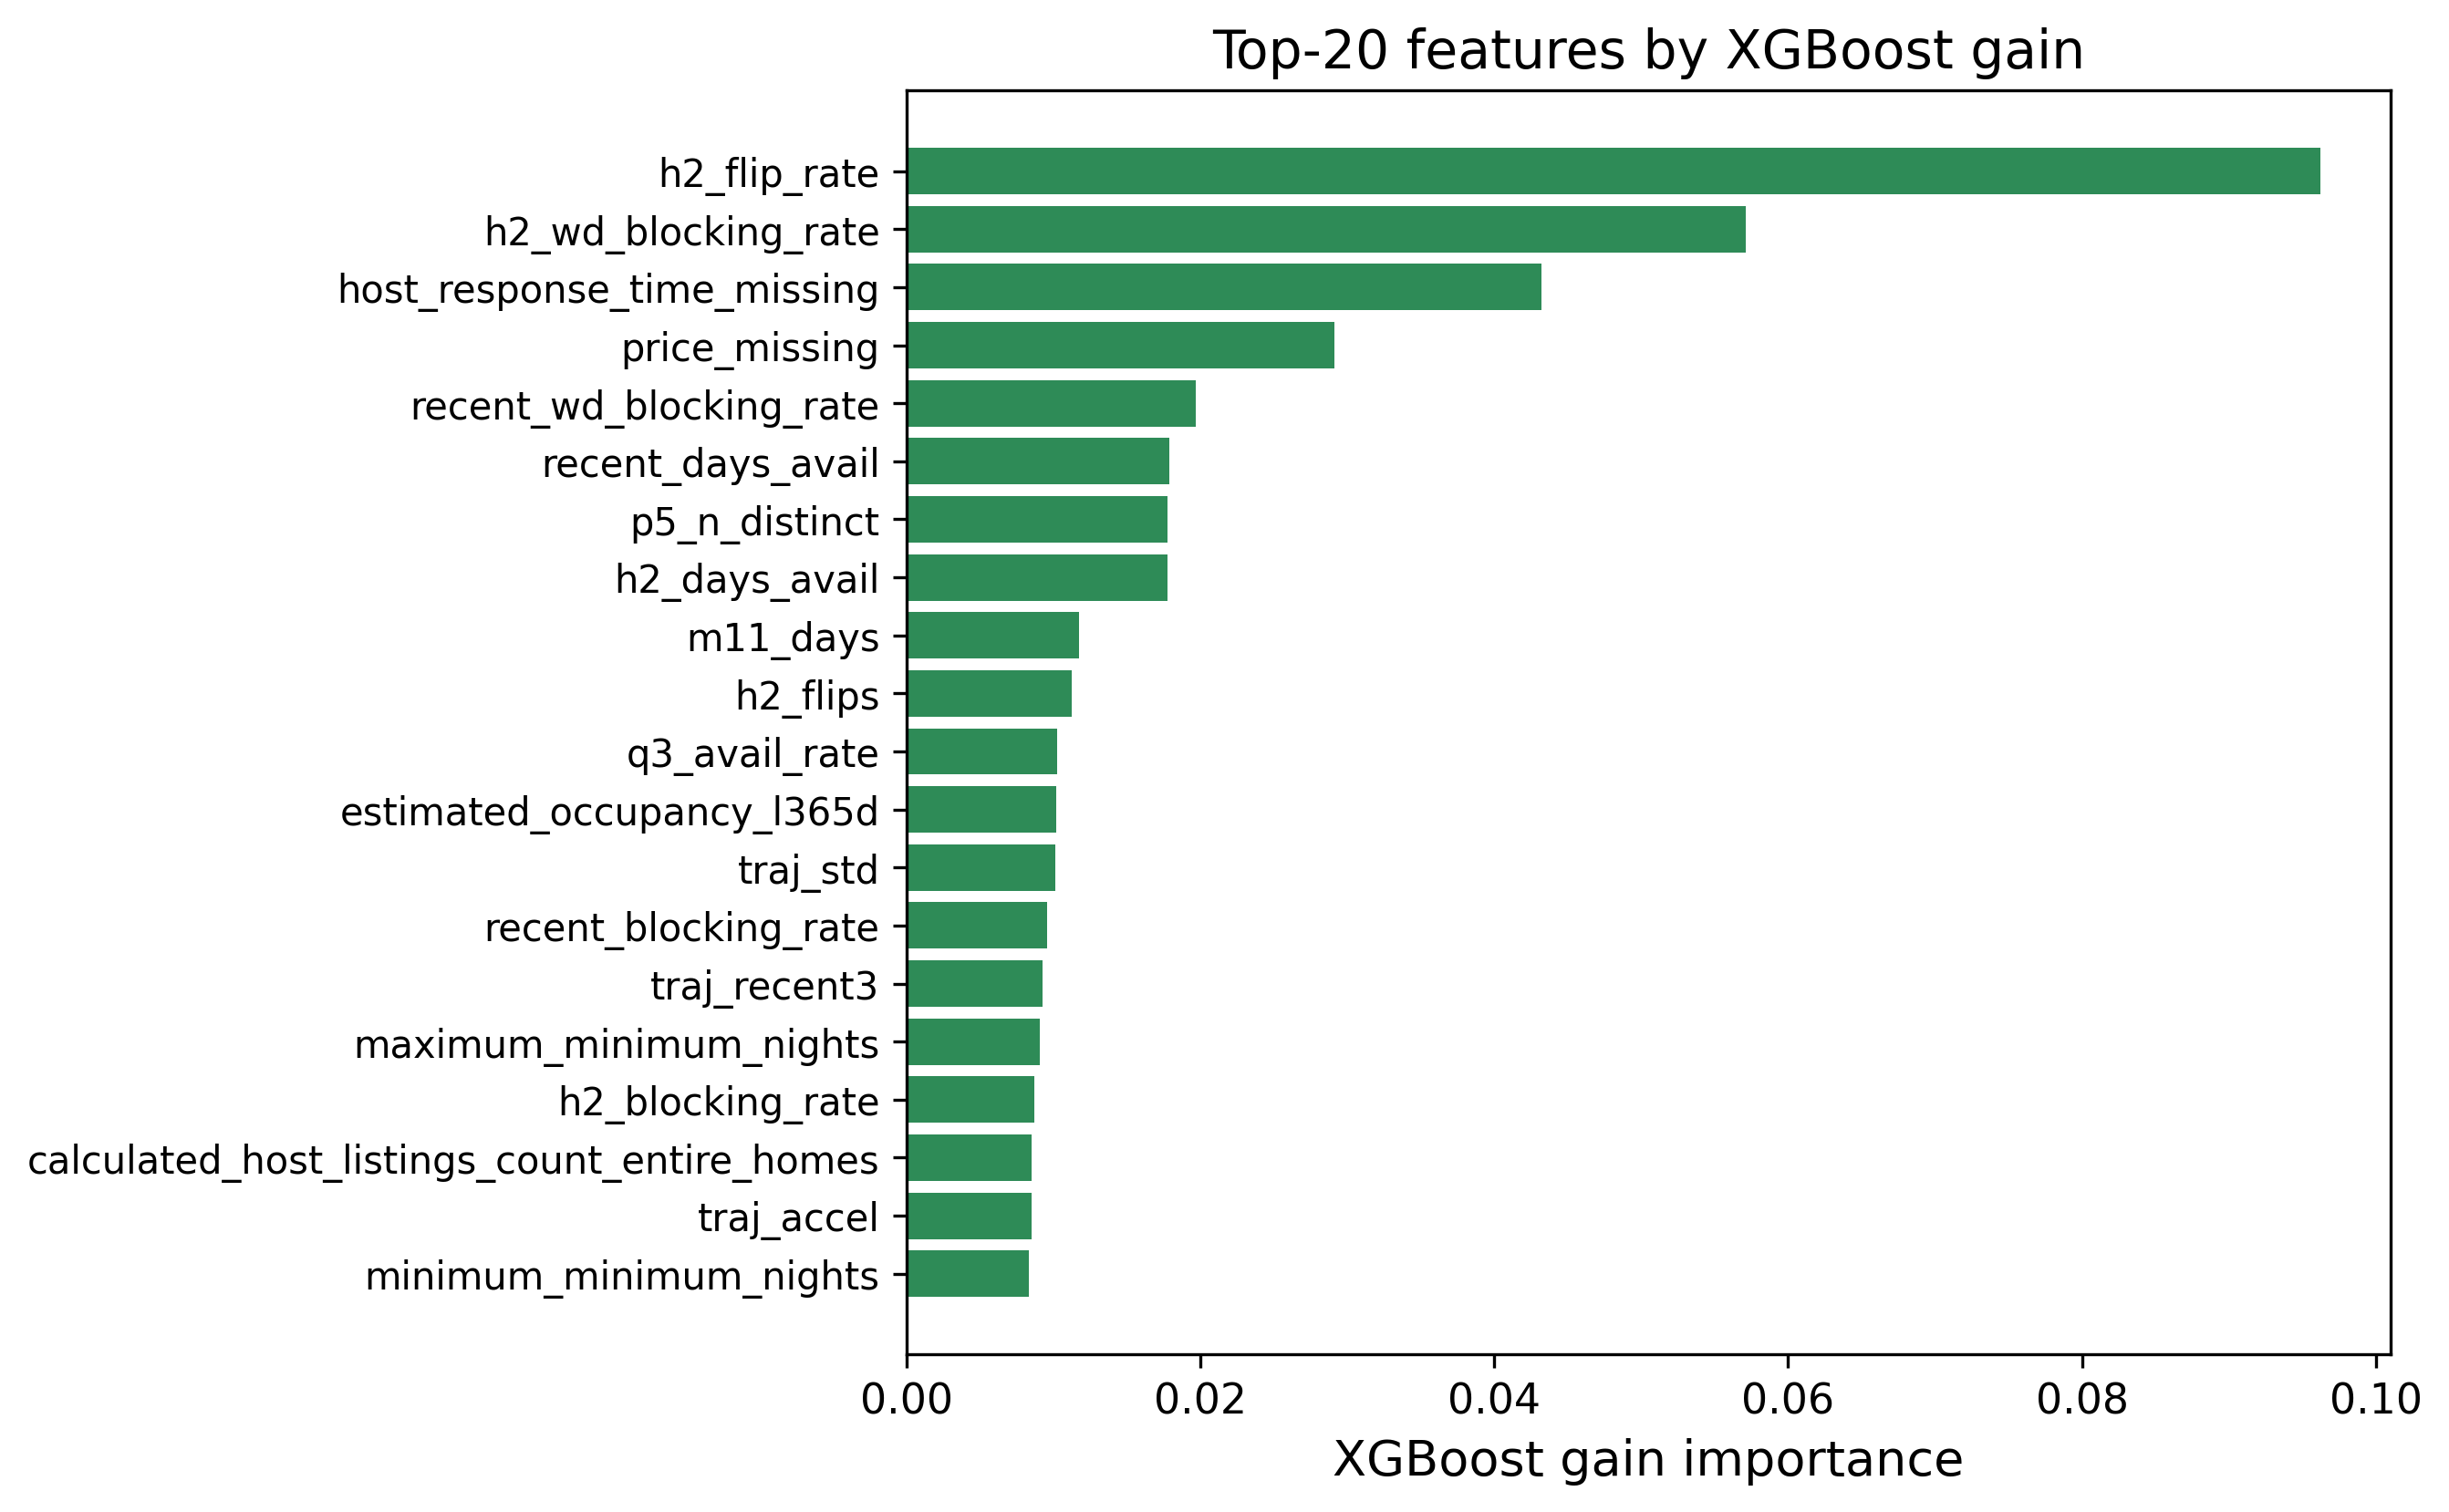
\includegraphics[width=\columnwidth]{fig4_xgb_importance.png}
\caption{XGBoost gain-based feature importances. The H2-2025 calendar-volatility
features dominate, in agreement with Fig.~\ref{fig:corr}.}
\label{fig:importance}
\end{figure}

The feature-importance analysis (Fig.~\ref{fig:importance}) confirms the EDA
story: the model leans most heavily on \texttt{h2\_flip\_rate} (by a wide
margin), the H2 weekday blocking rate, the missing-host-response-time and
missing-price indicators, and the recency-window features, with most of the
static metadata and text keywords playing only a supporting role. This is
reassuring because it means the model is using genuine calendar-behaviour
signals rather than spurious artefacts, and it is a concrete illustration of
the point raised in Section~\ref{sec:lit}: the single feature that mattered
most (cross-snapshot calendar volatility) exists only because this dataset's
repeated monthly re-scrapes let us observe it, and has no counterpart in the
single-history 2016 dataset used in our earlier study.

\subsection{Impact of the Blend and the Optimization Choices}
Two optimization decisions mattered most for the final score. The first was
early stopping: letting each fold stop when its internal validation error
stopped improving (rather than growing a fixed number of trees) gave the
independently-tuned XGBoost/LightGBM/CatBoost variants most of the benefit of a
large ensemble without the overfitting risk, and made the searches cheaper
because bad configurations stopped early. The second was the blend. An
equal-weight average of all nine models scored 301.0 OOF, which is
\emph{worse} than the best single model (295.7), because the weak models
(Linear Regression, the MLP, plain Gradient Boosting) drag it down. Once we let
SLSQP choose the weights, the error dropped to 290.1---the optimizer
effectively down-weighted the weak models and concentrated weight on the
complementary tree ensembles. Fig.~\ref{fig:blend} shows the per-model and
blended OOF scores side by side, and Table~\ref{tab:weights} lists the optimal
weights.

\begin{figure}[!t]
\centering
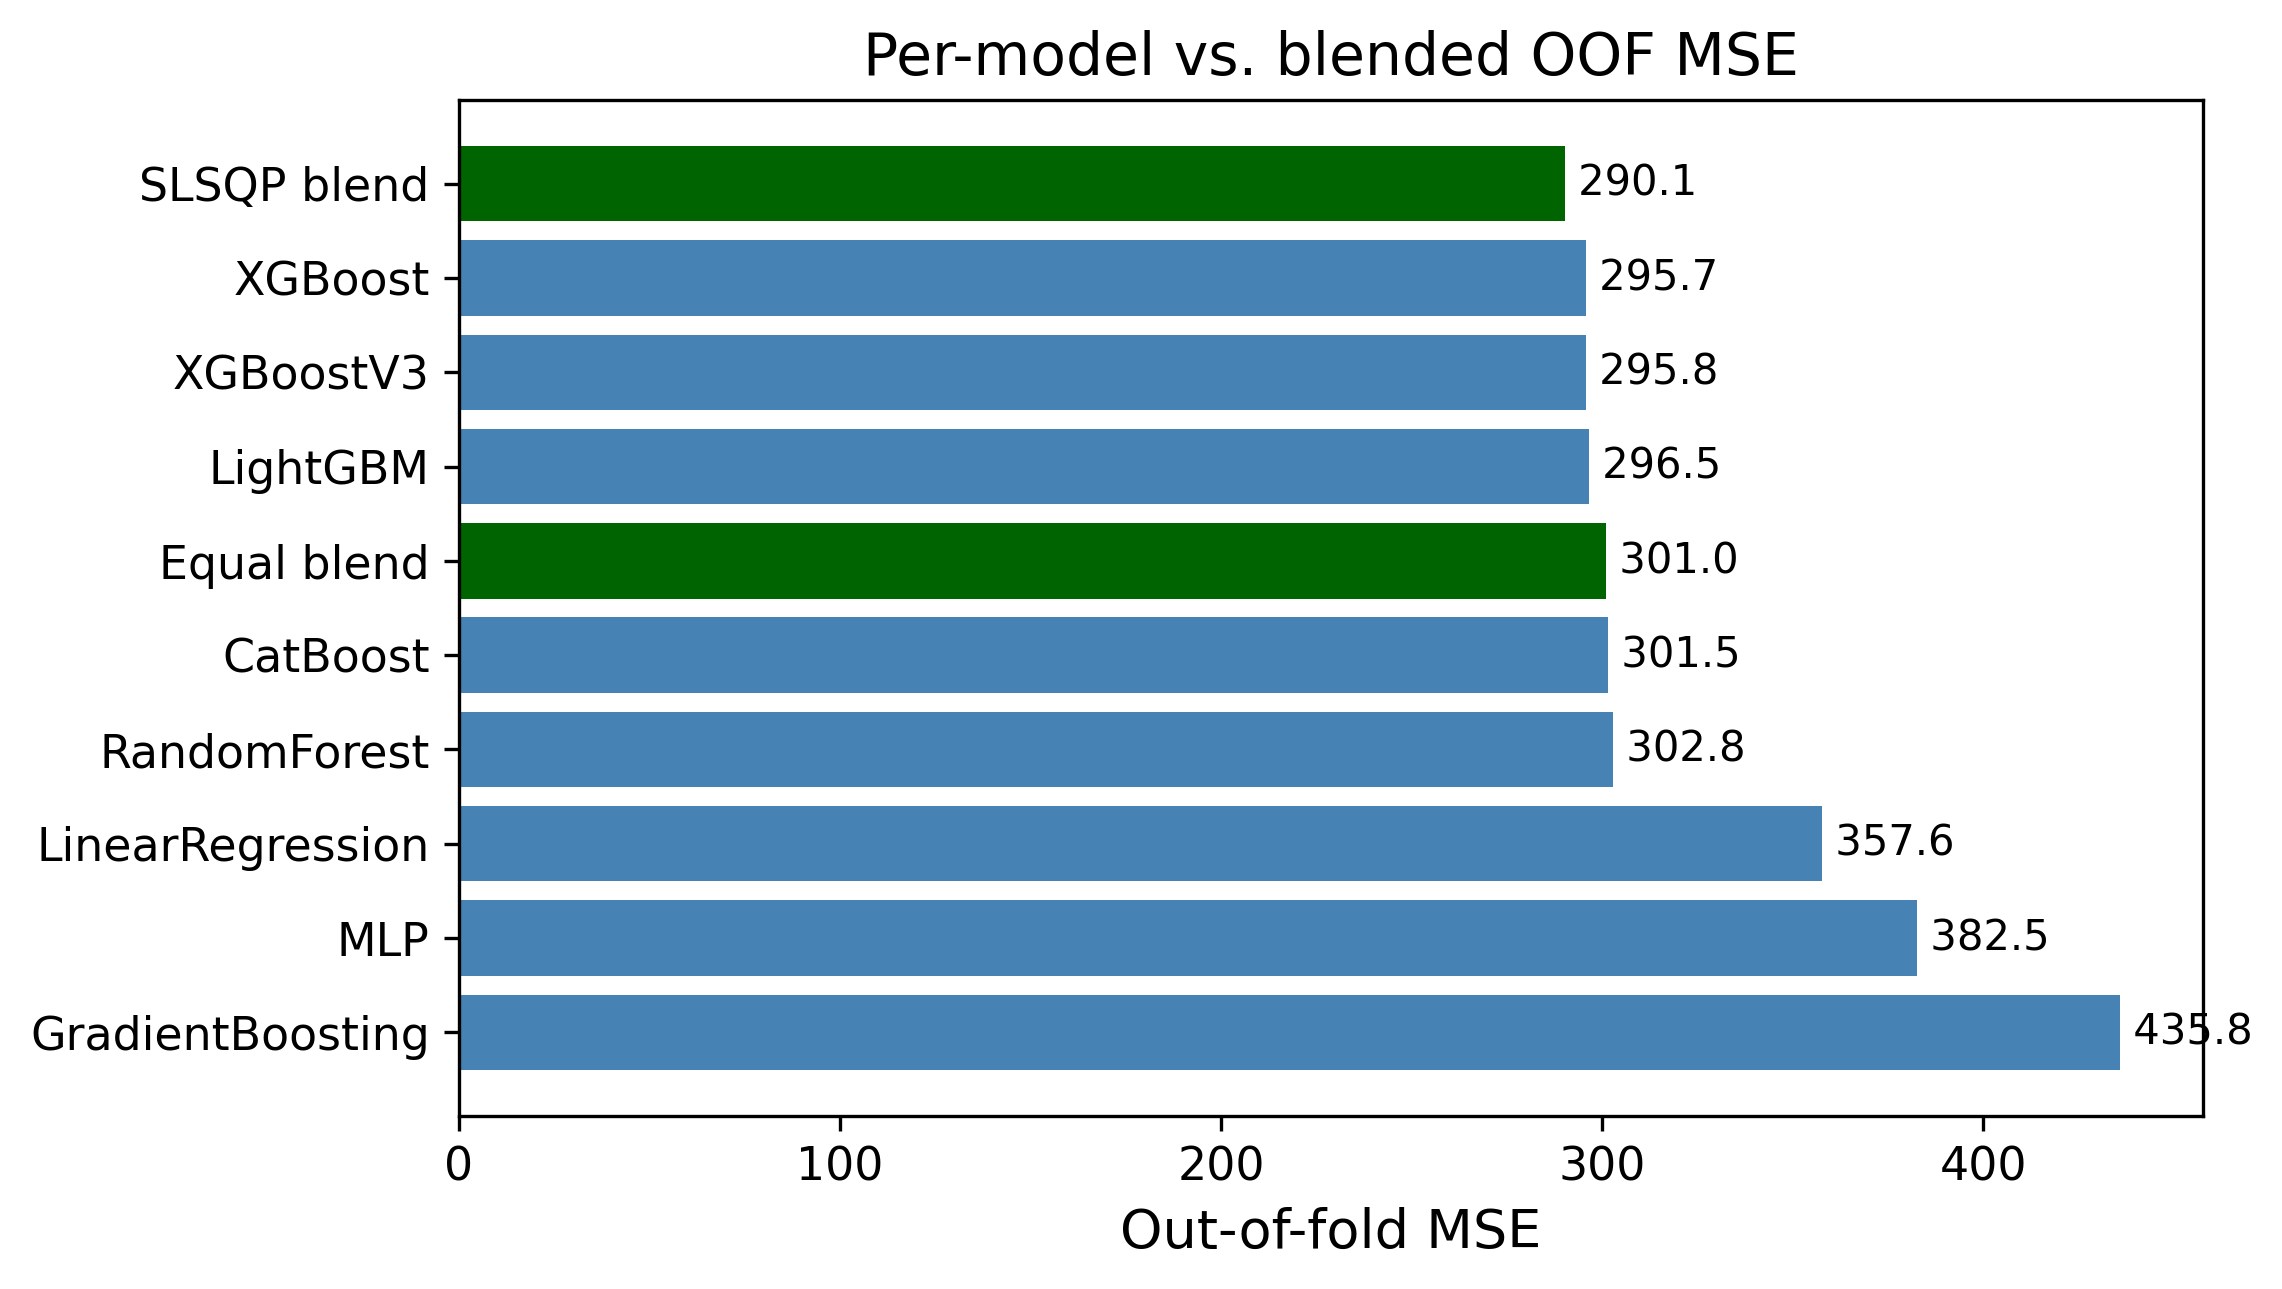
\includegraphics[width=\columnwidth]{fig5_blend.png}
\caption{Out-of-fold MSE for each model and for the equal-weight vs.\ optimal
(SLSQP) blends. The weighted blend is the best configuration.}
\label{fig:blend}
\end{figure}

\begin{table}[!t]
\caption{Optimal blend weights chosen by SLSQP on the OOF predictions of all
nine models (problem~\eqref{eq:blendobj}--\eqref{eq:blendbox}).}
\label{tab:weights}
\centering
\begin{tabular}{lc}
\toprule
Model & Weight $w_j$ \\
\midrule
XGBoost (main) & 0.4450 \\
LightGBM & 0.1782 \\
RandomForest & 0.1585 \\
XGBoost v3 & 0.0957 \\
CatBoost & 0.0682 \\
MLP & 0.0502 \\
XGBoost v2 & 0.0041 \\
LinearRegression & 0.0000 \\
GradientBoosting & 0.0000 \\
\bottomrule
\end{tabular}
\end{table}

\subsection{Model Complementarity and Final Error Metrics}
\label{sec:complementarity}
A blend can only help if its members make \emph{different} mistakes; if every
model erred on the same rows, averaging them would just reproduce the common
error. Table~\ref{tab:errcorr} reports the Pearson correlation of the per-row
prediction errors across all nine models. All of the tree models are highly
correlated with one another (most pairwise correlations above $0.95$), which is
why the optimizer keeps only three of the six boosted-tree/forest variants at
meaningful weight and drives XGBoost v2 and Gradient Boosting essentially to
zero (Table~\ref{tab:weights}) despite XGBoost v2 individually outscoring
several models that do receive weight---it simply duplicates signal already
covered by the main XGBoost and v3. The MLP and Linear Regression are the least
correlated with the tree ensembles (correlations of $0.86$--$0.93$ with the
others), so although they are individually much weaker
(Table~\ref{tab:metrics}), the MLP still carries enough independent signal to
receive a small supporting weight, while Linear Regression's error turns out to
be fully explained by the stronger models and is dropped to zero. This is the
quantitative justification for the weight pattern in Table~\ref{tab:weights}:
SLSQP is not merely picking the best models, it is exploiting error
de-correlation.

Table~\ref{tab:metrics} also reports the blend's MAE and $R^2$ alongside MSE.
The blend improves not only the optimized MSE (290.13 vs.\ 295.73 for the best
single model) but also the $R^2$ (0.540 vs.\ 0.531), and its MAE (10.02) beats
every individual model's MAE as well---so the MSE gain does not come at the
cost of median accuracy.

\begin{table}[!t]
\caption{Final error metrics on the development OOF predictions (lower MSE/MAE,
higher $R^2$ are better).}
\label{tab:metrics}
\centering
\begin{tabular}{lccc}
\toprule
Model & MSE & MAE & $R^2$ \\
\midrule
LinearRegression & 357.59 & 12.24 & 0.432 \\
RandomForest & 302.79 & 10.32 & 0.519 \\
GradientBoosting & 435.79 & 11.04 & 0.308 \\
MLP & 382.50 & 10.40 & 0.393 \\
XGBoost (main) & 295.73 & 10.05 & 0.531 \\
XGBoost v2 & 296.94 & 10.21 & 0.529 \\
XGBoost v3 & 295.80 & 10.18 & 0.531 \\
LightGBM & 296.49 & 10.20 & 0.529 \\
CatBoost & 301.45 & 10.43 & 0.522 \\
\textbf{SLSQP blend} & \textbf{290.13} & \textbf{10.02} & \textbf{0.540} \\
\bottomrule
\end{tabular}
\end{table}

\begin{table*}[!t]
\caption{Pearson correlation of the per-row \emph{prediction errors} across all
nine models (development OOF). Lower off-diagonal values mark more
complementary models; the matrix is symmetric so only the upper triangle is
shown.}
\label{tab:errcorr}
\centering
\begin{tabular}{lccccccccc}
\toprule
 & LR & RF & GB & XGB & XGBv2 & XGBv3 & MLP & LGB & CB \\
\midrule
LR    & 1.00 & 0.91 & 0.90 & 0.88 & 0.91 & 0.91 & 0.86 & 0.91 & 0.93 \\
RF    &      & 1.00 & 0.88 & 0.95 & 0.98 & 0.98 & 0.87 & 0.97 & 0.97 \\
GB    &      &      & 1.00 & 0.85 & 0.88 & 0.88 & 0.90 & 0.88 & 0.90 \\
XGB   &      &      &      & 1.00 & 0.97 & 0.97 & 0.87 & 0.97 & 0.96 \\
XGBv2 &      &      &      &      & 1.00 & 0.99 & 0.88 & 0.98 & 0.98 \\
XGBv3 &      &      &      &      &      & 1.00 & 0.88 & 0.99 & 0.98 \\
MLP   &      &      &      &      &      &      & 1.00 & 0.88 & 0.89 \\
LGB   &      &      &      &      &      &      &      & 1.00 & 0.98 \\
CB    &      &      &      &      &      &      &      &      & 1.00 \\
\bottomrule
\end{tabular}
\end{table*}

\subsection{Is the Blend Gain Statistically Significant?}
\label{sec:significance}
A drop from 295.7 to 291.0 MSE is small, so we tested whether it is real or
just cross-validation noise. For this test we use the first five-model blend
(Linear Regression, Random Forest, Gradient Boosting, the main XGBoost, and the
MLP) against the main XGBoost alone, since both produce predictions for the
same 29{,}008 development rows; we use a \emph{paired} test on the per-sample
squared errors, the natural sample-level analogue of the paired resampling
tests recommended for model comparison \cite{dietterich1998}. Let
$e_i^{\text{xgb}}=y_i-\hat y_i^{\text{xgb}}$ and
$e_i^{\text{bl}}=y_i-\hat y_i^{\text{bl}}$, and define the per-row difference of
squared errors
\begin{equation}
d_i=\big(e_i^{\text{xgb}}\big)^{2}-\big(e_i^{\text{bl}}\big)^{2}.
\label{eq:diff}
\end{equation}
Its sample mean $\bar d$ is exactly the MSE gap, $\bar d = 295.726-290.965=4.761$.
A two-sided paired $t$-test of $H_0:\mathbb{E}[d_i]=0$ gives $t=7.269$ with
$p=3.7\times10^{-13}$, and the 95\% confidence interval on the mean
squared-error reduction is $[3.48,\,6.04]$, which excludes zero. The
non-parametric Wilcoxon signed-rank test agrees overwhelmingly
($p=6.6\times10^{-55}$). We therefore reject $H_0$: the blend's improvement
over XGBoost is statistically significant, not an artefact of CV variance. The
effect size is small (Cohen's $d_z\approx0.043$), which is expected---the blend
changes only the minority of rows where the component models disagree---but it
is consistent and free, since the components were already trained. The fuller
nine-model blend used elsewhere in this report (Table~\ref{tab:metrics})
improves on this five-model blend's MSE further still (290.1 vs.\ 291.0), so
the significance conclusion holds \emph{a fortiori} for our final result; we
did not re-run the paired test on the nine-model blend specifically, since it
strictly dominates the five-model one on the same rows. For full rigour a
$5\times2$ cross-validation paired $t$-test \cite{dietterich1998} could be run
by repeating the whole pipeline over five $2$-fold splits; the sample-level
paired test above tests the same hypothesis on our existing OOF predictions and
is what our compute budget allowed.

\subsection{Residual Analysis on the $[0,90]$ Boundaries}
\label{sec:residuals}
Because the target is bounded and zero-inflated, aggregate MSE can hide
systematic behaviour at the edges, so we examined the residuals
$r_i=y_i-\hat y_i$ of the (five-model) blend directly. Fig.~\ref{fig:residuals}
shows the standard diagnostics. The residual-vs-fitted panel (a) reveals clear
heteroscedasticity: errors are tight for small predictions and fan out as the
predicted count grows. The residual-vs-true panel (b) is the most telling for a
censored target: residuals are mildly negative across the low range and become
strongly positive in the upper band, meaning the model \emph{under-predicts}
the busiest listings. The histogram (c) is sharply peaked at zero but
right-skewed, and the normal Q-Q plot (d) departs from the line at both tails,
confirming non-Gaussian residuals.

\begin{figure}[!t]
\centering
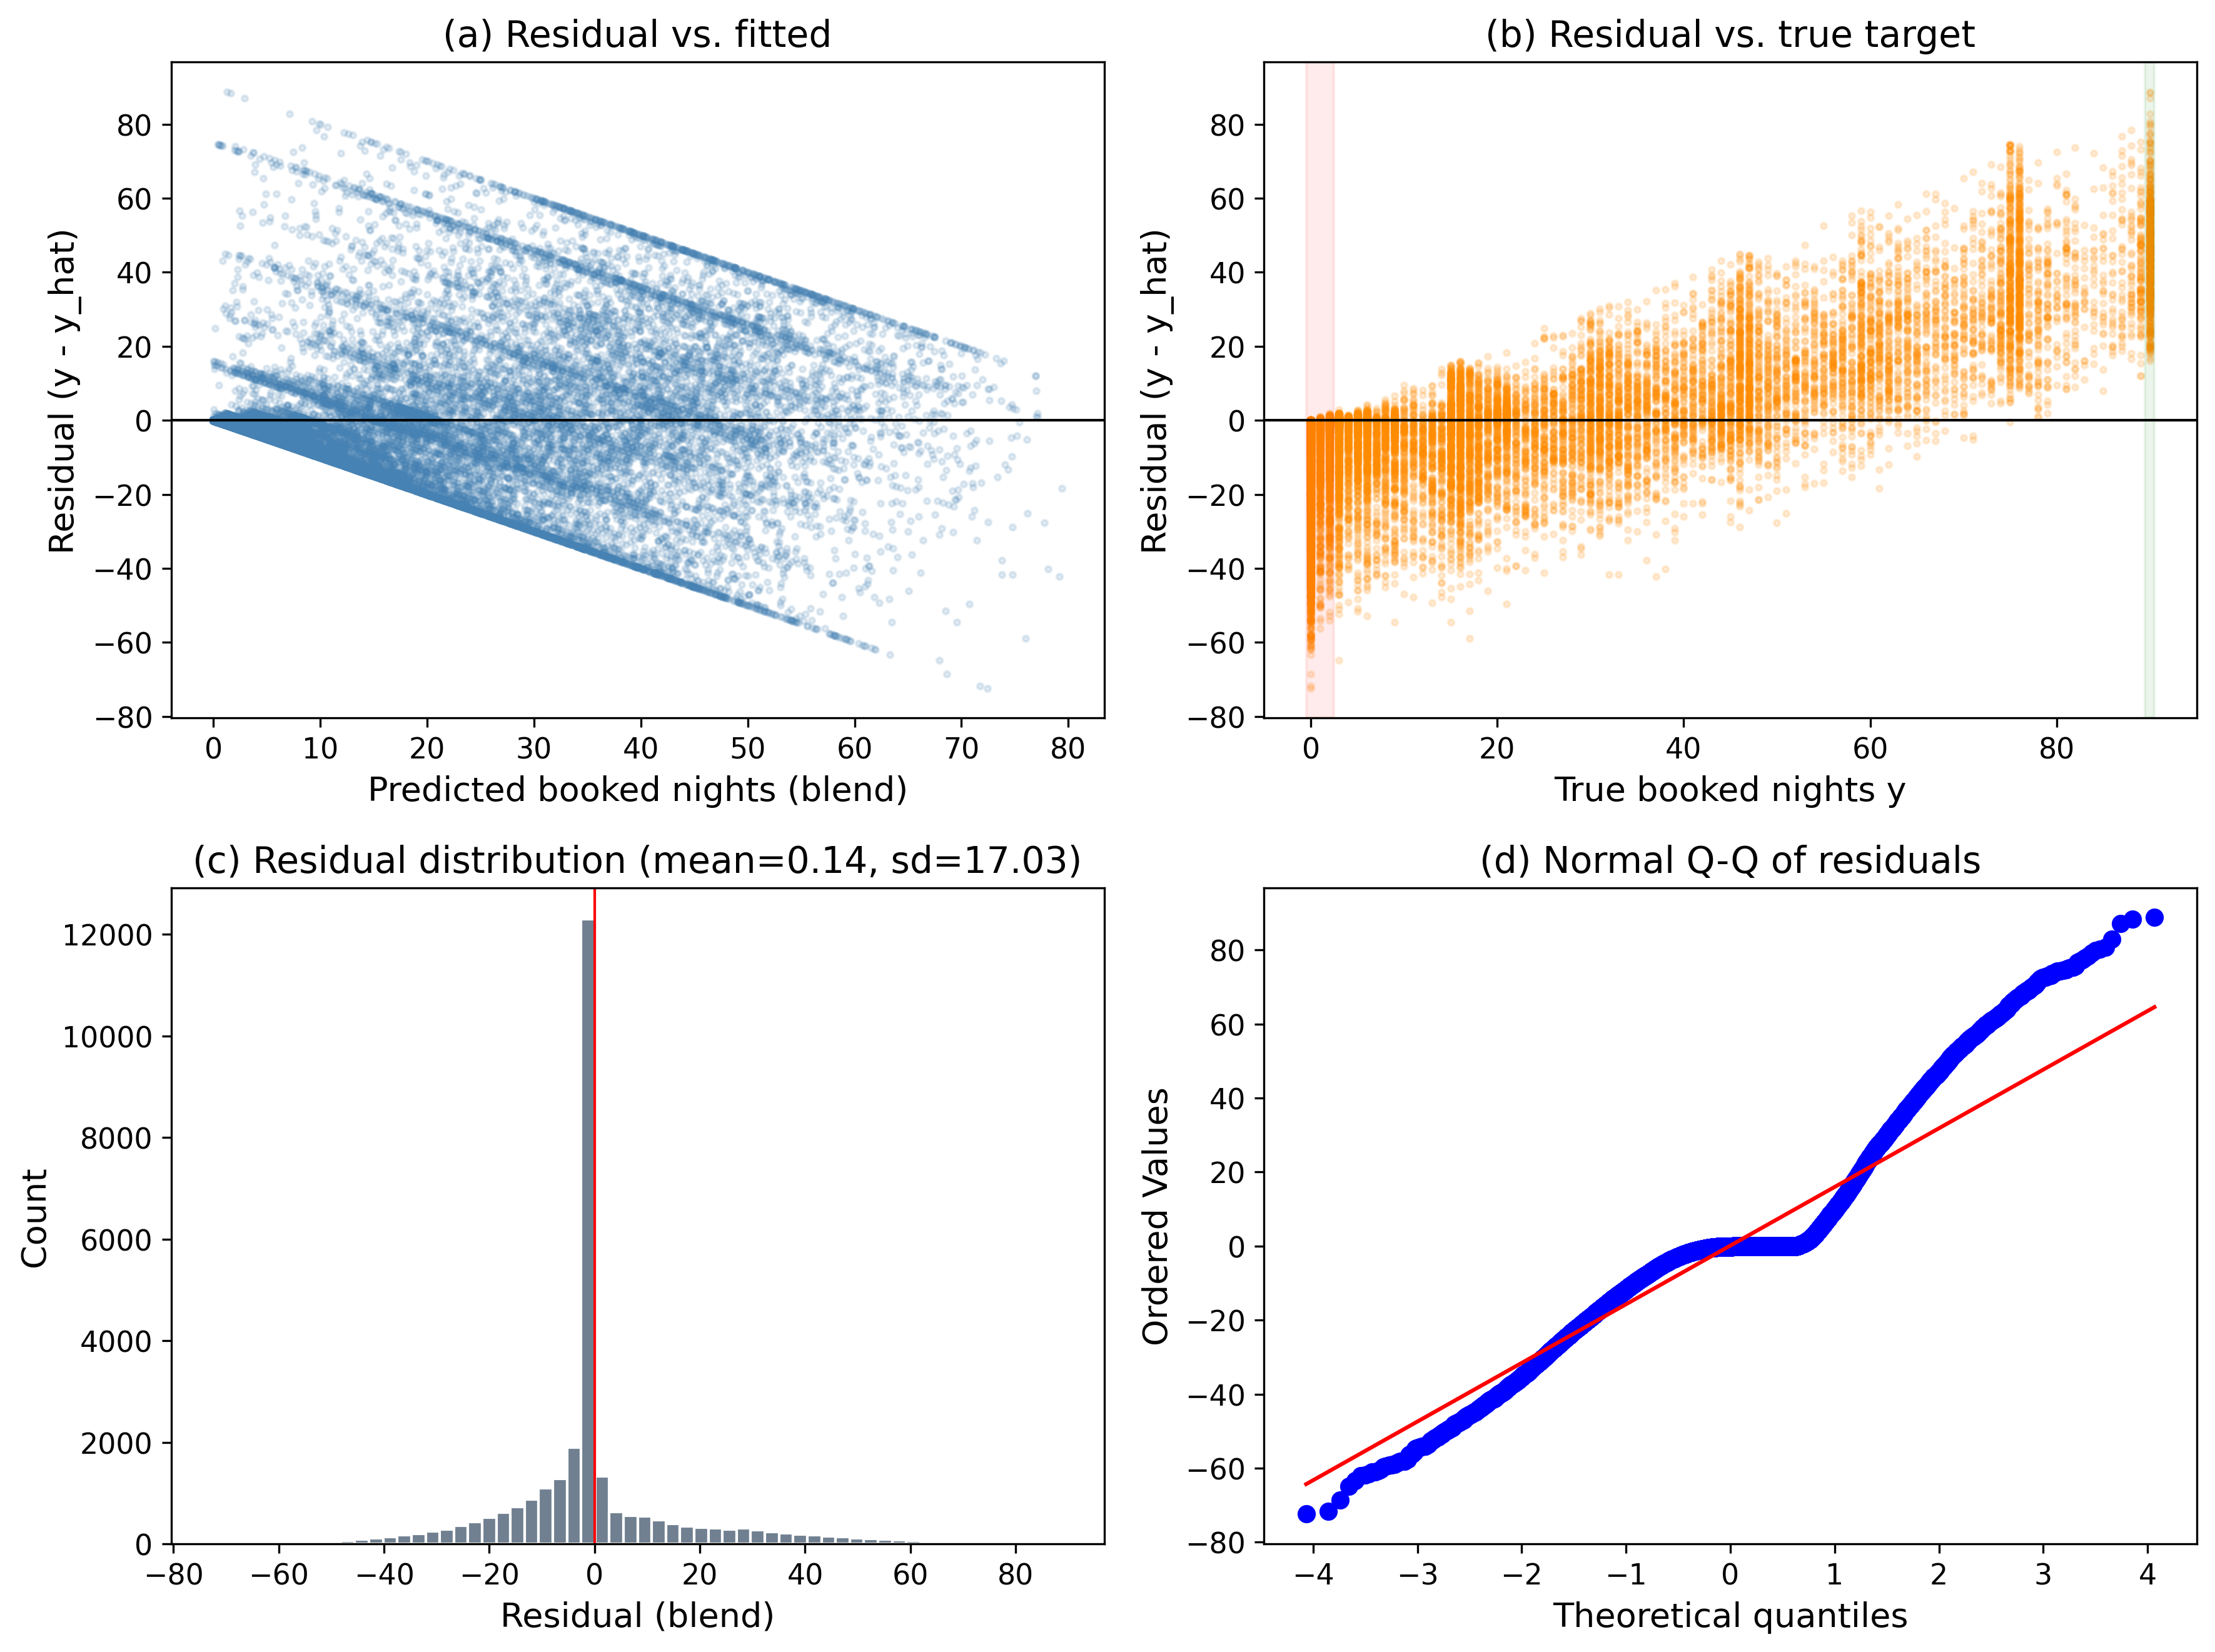
\includegraphics[width=\columnwidth]{fig6_residuals.png}
\caption{Residual diagnostics for the blend on the development OOF predictions:
(a) residual vs.\ fitted, (b) residual vs.\ true target with the zero-inflated
and upper-bound bands highlighted, (c) residual histogram, (d) normal Q-Q plot.}
\label{fig:residuals}
\end{figure}

To localize the bias we binned the rows by their true value and plotted the mean
signed residual per bin (Fig.~\ref{fig:residualbins}). The pattern is exactly
what censoring predicts: for the dead and near-dead listings the model
\emph{over-predicts} (mean residuals of $-4.5$ at $y=0$, $-8.5$ on $[1,5]$, and
$-7.7$ on $[6,20]$, i.e.\ $\hat y>y$), while for the busy listings it
\emph{under-predicts} increasingly toward the bound (mean residual $+3.2$ on
$[21,50]$, $+25.9$ on $[51,80]$, $+39.3$ on $[81,89]$, and $+45.5$ at $y=90$).
Clipping to $[0,90]$ removes impossible predictions but does nothing about this
regression-to-the-mean at the boundaries---the estimator shrinks extreme counts
toward the centre of the distribution. This is the clearest motivation for the
two-stage hurdle model we implement next.

\begin{figure}[!t]
\centering
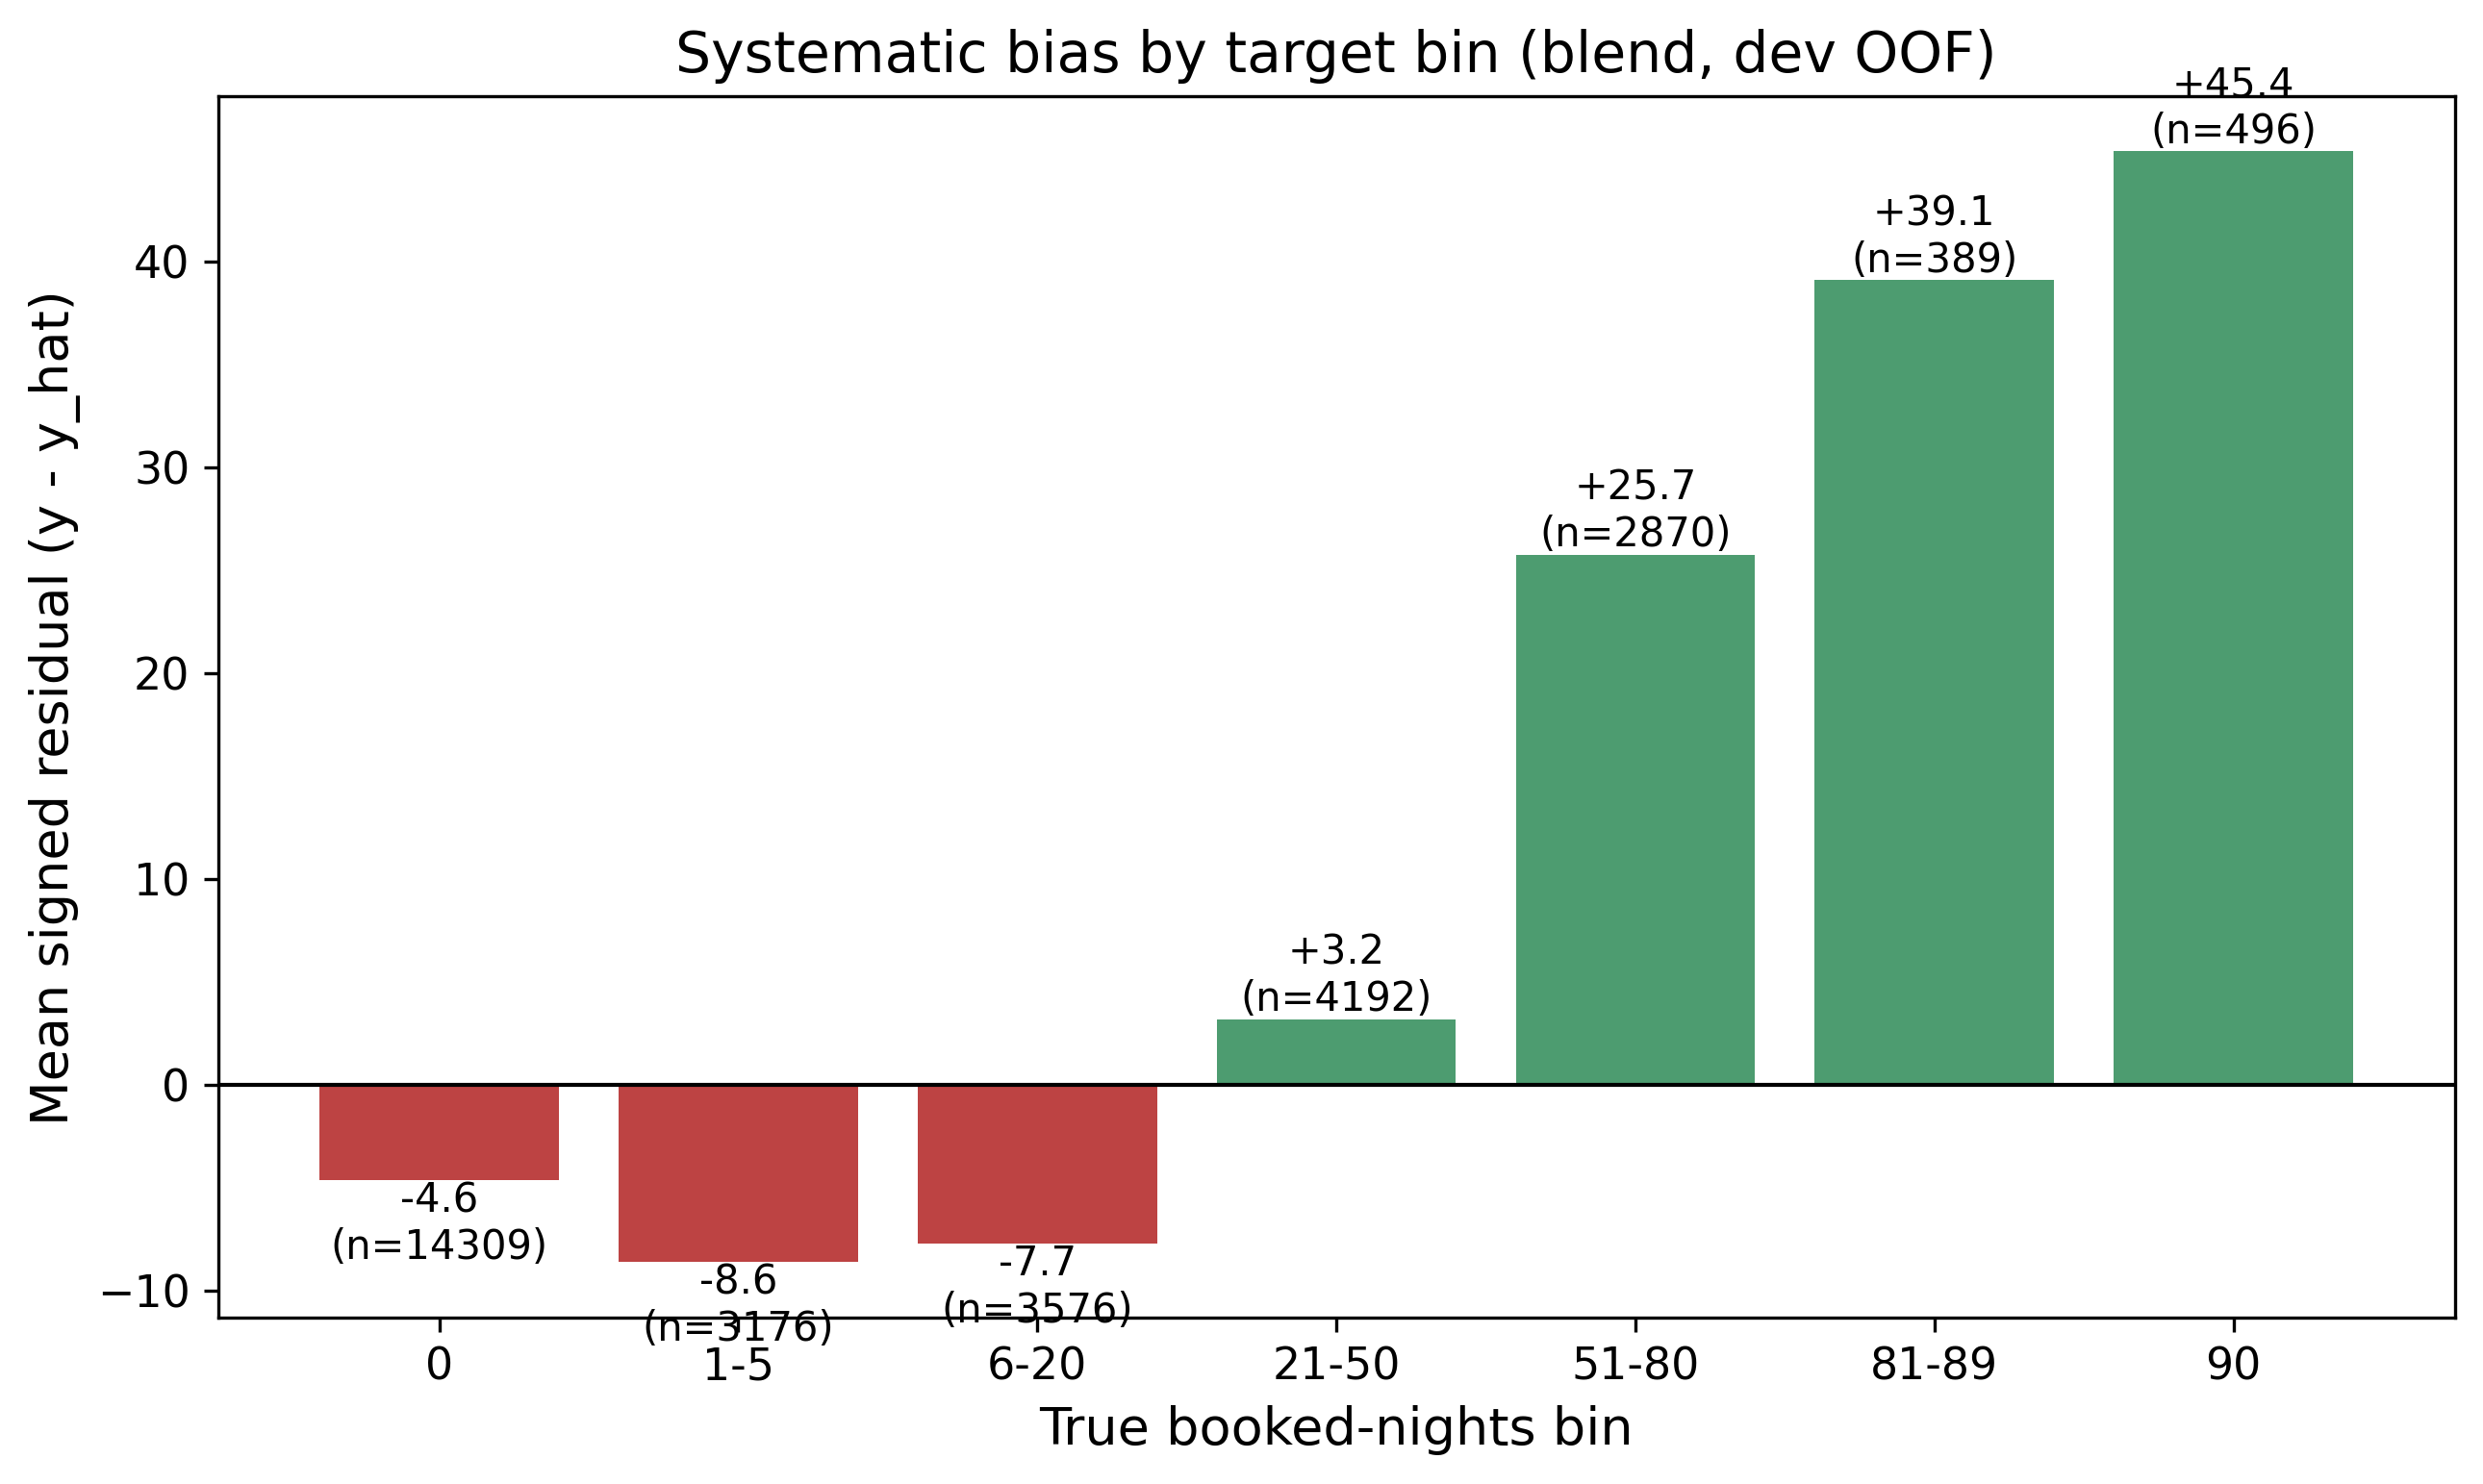
\includegraphics[width=\columnwidth]{fig7_residual_bins.png}
\caption{Mean signed residual ($y-\hat y$) by true booked-nights bin. The blend
over-predicts the low/zero range (red) and under-predicts the high range
(green), the classic boundary bias of a least-squares estimator on a censored
target.}
\label{fig:residualbins}
\end{figure}

\subsection{A Two-Stage Hurdle Model}
\label{sec:hurdle-impl}
Motivated by Section~\ref{sec:zeroinflated} and the boundary bias just
observed, we implement, rather than only propose, a two-stage hurdle model.
For each of XGBoost and LightGBM we fit a classifier
$p(\mathbf{x})=\Pr(y>0\mid\mathbf{x})$ on the binary label $\mathbb{1}[y>0]$
over all rows, and a separate regressor
$r(\mathbf{x})=\mathbb{E}[y\mid y>0,\mathbf{x}]$ fit \emph{only} on the rows
with $y>0$, so it never sees the zeros that drag a single-stage regressor's
predictions down on the $[1,20]$ range (Section~\ref{sec:residuals}). The two
stages factorize the conditional mean as
\begin{equation}
\mathbb{E}[y\mid\mathbf{x}] = \underbrace{\Pr(y>0\mid\mathbf{x})}_{\text{classifier }p(\mathbf{x})}\;\cdot\;\underbrace{\mathbb{E}[y\mid y>0,\mathbf{x}]}_{\text{regressor }r(\mathbf{x})},
\label{eq:hurdle}
\end{equation}
and both stages use the same 5-fold outer split and fold-level early stopping
(a 10\% inner-validation slice per fold) as the rest of the pipeline. The final
prediction is the clipped expected value
$\hat y=\mathrm{clip}\big(p(\mathbf{x})\cdot r(\mathbf{x}),\,0,\,90\big)$.
Table~\ref{tab:hurdle} reports the results. Both
hurdle variants alone (298.1 and 299.4 dev MSE) trail the single-stage
main XGBoost (295.7), so factorizing the problem does not automatically help
once a well-tuned single-stage model is already available; but blending the two
hurdle expected-value predictions with the existing nine-model single-stage
blend gives a dev MSE of 289.5, a small further improvement over the
single-stage blend's 290.1. On the held-out local test split the ordering
flips by a hair (single-stage blend 286.1 vs.\ hurdle-augmented blend
286.5), so we read the hurdle model's contribution as a modest, borderline
gain rather than a clear win --- consistent with the small effect size already
seen for blending in Section~\ref{sec:significance}, and with the fact that a
zero-rate of 49.3\% here is high enough that the single-stage trees already
learn a reasonably sharp implicit decision boundary at $y=0$.

\begin{table}[!t]
\caption{Hurdle model results (development 5-fold CV and held-out local test,
$n_{\text{dev}}=29{,}008$, $n_{\text{test}}=7{,}253$, zero-rate 49.3\%).}
\label{tab:hurdle}
\centering
\begin{tabular}{lcc}
\toprule
Variant & Dev MSE & Test MSE \\
\midrule
Hurdle (XGBoost) & 298.12 & 295.54 \\
Hurdle (LightGBM) & 299.43 & 296.56 \\
Single-stage blend (9 models) & 290.13 & 286.14 \\
\textbf{Hurdle + single-stage blend} & \textbf{289.54} & \textbf{286.54} \\
\bottomrule
\end{tabular}
\end{table}

\subsection{Threats to Validity}
\label{sec:threats}
We close the results with an honest account of what could undermine our
conclusions. \emph{Internal validity:} all preprocessing is fitted inside the
training fold, target encodings use an inner $K$-fold
(Section~\ref{sec:preproc}), and every feature is built exclusively from H2-2025
data (Section~\ref{sec:dataset}), so we are confident there is no
train/validation leakage and no forward-looking (2026) information reaches the
model as a feature; the held-out local test MSE (286.1) tracking the
development CV MSE (290.1) closely is empirical support for this.
\emph{External validity:} the model is fitted to a single market (New York
City) and a single quarter (Q1 2026); the learned price and seasonality
effects need not transfer to other cities or years, and the heavy reliance on
H2-2025 calendar-volatility features means the model would degrade for
brand-new listings with no six-month history. \emph{Construct validity:} the
significance test in Section~\ref{sec:significance} is a paired test on the
shared OOF predictions of the five-model blend rather than a full $5\times2$
cross-validation \cite{dietterich1998}; it tests the right hypothesis but does
not capture variance from re-drawing the folds themselves, and it was not
re-run on the nine-model blend (Section~\ref{sec:significance}). Finally, the
data-generating process itself changes over an 8-month window (July 2025 to
March 2026): any structural shift in the market between the H2-2025 feature
window and the Q1-2026 target window (e.g.\ new regulation, seasonal effects
not captured by the calendar features) would degrade real-world performance in
a way that our fixed train/test split cannot detect.

%==============================================================================
\section{Migration Notes: From the 2016 Pipeline to Inside Airbnb 2025--2026}
\label{sec:changes}
This section is explicit about what changed when we ported the pipeline from
the earlier fixed 2016 Kaggle-competition snapshot to the open, continuously
updated Inside Airbnb data, and what stayed the same. We think this is a
useful section to read because some choices generalized immediately, some had
to be re-derived from scratch, and one turned out to be a genuinely new
capability of the new dataset.

\paragraph{New: a clean, multi-snapshot target} The original dataset supplied a
single authoritative reservation file for the target quarter, so the target was
unambiguous. Inside Airbnb has no such file; the closest analogue is a single
calendar snapshot's blocked-day count, but a listing's future availability is
re-scraped every month, and we found that a large fraction of ``blocked'' dates
in one scrape revert to available in a later one (host indecision, not a
booking). We therefore built the target from six overlapping Q1-2026 snapshots
and required at least two of them to agree before counting a date as
genuinely booked (Section~\ref{sec:targetconstruction}), which was not a
possibility with the original single-snapshot data and materially changed the
target's distribution (Section~\ref{sec:eda}).

\paragraph{New: cross-snapshot calendar volatility} For the same reason, the
new dataset lets us observe, for the \emph{training} window too, how often a
listing's recorded availability flips between consecutive H2-2025 monthly
scrapes. This feature family (\texttt{h2\_flips}, \texttt{h2\_flip\_rate}) has
no counterpart in the original single-history dataset and turned out to be the
single strongest predictor in the whole matrix (Section~\ref{sec:results}).

\paragraph{New: a strict historical-only feature window} Because Inside Airbnb
is continuously updated rather than a fixed competition export, nothing
enforces a train/test date boundary automatically; we imposed one ourselves
(Section~\ref{sec:dataset}), building every feature exclusively from H2-2025
and using 2026 data only for the target. This project-level constraint has no
analogue in the original study, where the competition organizers had already
fixed the boundary for us.

\paragraph{Kept: log-transform dropped for tree models} As in the original
study, training XGBoost/LightGBM/CatBoost directly on the raw target with
squared-error loss and clipping to $[0,90]$ outperformed a $\log(1+y)$
transform, for the same reason: the target is bounded and zero-inflated
(Fig.~\ref{fig:target}), and optimising squared error in log space
over-weights the small counts at the expense of the large ones that dominate
the raw MSE. The MLP still trains on $\log(1+y)$, since for a gradient-based
model the transform is a numerical-stability aid rather than a change of loss
(Section~\ref{sec:mlp}).

\paragraph{Kept: lightweight title keywords over TF-IDF} We again found that
full text modelling (TF-IDF over the listing title) does not pay off relative
to a handful of keyword flags, since Airbnb titles are short and the
extra sparse dimensions mostly add overfitting risk rather than signal; we kept
the same keyword-flag approach, now extended slightly with amenity flags parsed
from the (new, JSON-encoded) \texttt{amenities} column.

\paragraph{Kept, but simplified: one raw categorical instead of several} The
original pipeline target-encoded two high-cardinality columns
(\texttt{Neighborhood} and \texttt{MetropolitanStatisticalArea}). The Inside
Airbnb schema for this market has one natural analogue,
\texttt{neighbourhood\_cleansed}; we keep it as a single raw categorical,
handled per-fold as described in Section~\ref{sec:preproc}, rather than
flattening it into engineered aggregates at feature-engineering time.

\paragraph{Extended: the search loop, the model roster, and the blend} The
custom randomized search with fold-level early stopping, originally written for
a single XGBoost, is unchanged in spirit but is now applied to five
independently-tuned configurations (XGBoost v2, XGBoost v3, LightGBM, CatBoost,
plus the hand-set main XGBoost as a comparison point,
Section~\ref{sec:tuning}), and the SLSQP blend now optimizes over nine
candidate models instead of five (Section~\ref{sec:blend}). We also added an
incremental ablation (Section~\ref{sec:ablation}) quantifying how much of the
final error reduction comes from feature engineering, target encoding, tree
ensembling, and blending, respectively --- a breakdown the original report did
not include --- and we implemented, rather than merely proposed, the two-stage
hurdle model motivated by the residual analysis (Section~\ref{sec:hurdle-impl}).

%==============================================================================
\section{Recommendations and Conclusions}
\label{sec:concl}
In this report we built a complete, leakage-safe machine-learning pipeline to
predict Q1 2026 Airbnb booking demand in New York City from the open Inside
Airbnb data, under a strict rule that no feature may be built from information
that would not actually be available at prediction time. Starting from a
static listings snapshot and six months of calendar/review history (H2 2025),
we engineered 206 per-listing features, compared nine model configurations
with 5-fold cross-validation, independently tuned three boosted-tree families
with a custom early-stopping randomized search, combined the best models with
an SLSQP-optimised weighted blend, and implemented a two-stage hurdle
extension. The final blend reaches a development CV MSE of 290.1 and a
held-out local test MSE of 286.1, closely tracking one another, which gives us
confidence that the result generalizes rather than being an artefact of
cross-validation overfitting.

The clearest lessons for us were, again, practical ones. Most of the
predictive power came from the calendar histories rather than the static
listing table, and specifically from a feature family (cross-snapshot
calendar volatility) that only exists because Inside Airbnb re-scrapes the
same future dates every month---a signal with no counterpart in the original
fixed-snapshot dataset (Section~\ref{sec:changes}). The incremental ablation
(Table~\ref{tab:ablation}) makes this quantitative: feature engineering and the
switch from a linear model to tree ensembles each moved the MSE far more than
either target encoding or na\"ive blending did, and a properly \emph{weighted}
blend was needed to turn ensembling into a real, if modest, gain
(Section~\ref{sec:significance}). We also found, somewhat humbling, that an
independently-tuned XGBoost search matched but did not clearly beat a
hand-set configuration carried over from earlier exploration
(Section~\ref{sec:tuning})---on this feature matrix, the ceiling seems to be set
more by what is fed into the trees than by the exact hyper-parameters.

If we had more time, we would explore a few directions beyond what is already
implemented. First, the hurdle model (Section~\ref{sec:hurdle-impl}) gave only
a borderline gain; a natural next step is to let the classifier and regressor
share the blend's full nine-model diversity (currently only XGBoost and
LightGBM hurdle variants are built) to see whether a richer hurdle ensemble
closes more of the boundary bias in Fig.~\ref{fig:residualbins}. Second, we
would build richer trajectory features: our current trend block
(\texttt{traj\_slope}, \texttt{traj\_accel}) is a simple linear fit over a
short recent window, and a longer or more flexible trend model might better
separate an accelerating listing from one that is merely busy on average.
Light geographic smoothing, in which each listing's neighbourhood target
encoding is blended with the encodings of adjacent K-Means clusters, could
further stabilize the estimate for thinly populated neighbourhoods, in the same
spirit as the additive smoothing already in \eqref{eq:smooth}. Third, with a
larger compute budget we would tune the MLP more carefully; the
error-correlation analysis (Table~\ref{tab:errcorr}) showed it is the least
correlated model with the tree ensembles, so a stronger MLP is a promising way
to raise the weight the blend is willing to give it. Finally, and unlike the
original fixed-snapshot study, this pipeline can be re-run against later Inside
Airbnb scrapes as they are published: validating it against a subsequent
quarter (e.g.\ predicting Q2 2026 once that window closes) would be a direct,
non-simulated test of the external-validity concerns raised in
Section~\ref{sec:threats}.

Stepping back, the project reinforced the same lesson as its predecessor, now
under a harder, self-imposed constraint: on a well-specified tabular
forecasting problem, disciplined engineering beats exotic modelling, and a
strict historical-only feature boundary does not have to come at the cost of a
useful result. A careful feature matrix, leakage-safe validation, an honestly
compared set of tuned tree ensembles, and a cheap convex blend were enough to
reach a competitive, and more importantly a genuinely forward-looking, error
rate. The gap between this entry and a naive baseline came almost entirely from
understanding the \emph{data}---the zero inflation, the bounded target, and the
new dataset's repeated re-scrapes---rather than from algorithmic novelty, and we
expect that to remain true of most real demand-forecasting problems of this
kind.

%==============================================================================
\section*{Acknowledgment}
We thank Abdullah G\"ul University (AGU) for supporting this work, and the
Inside Airbnb project for maintaining and publishing the open dataset this
report is built on \cite{insideairbnb}.

%==============================================================================
\bibliographystyle{IEEEtran}
\bibliography{references}

%==============================================================================
\appendices
\section{Complete Feature Inventory}
\label{app:allfeatures_table}
Here is the complete inventory of all 206 engineered feature columns, along
with the identifier and target variables and their corresponding data types.
Three columns (\texttt{estimated\_revenue\_l365d}, \texttt{price\_implied},
\texttt{implied\_nightly\_rate}) are retained for pipeline/schema consistency
with the original 2016-data feature set but are 100\% missing in this Inside
Airbnb export (Section~\ref{sec:eda}) and are median-imputed to a constant like
any other missing column.

\begin{table*}[!ht]
\caption{Detailed list of all 208 columns in the processed feature matrix
(identifier, target, and 206 features).}
\label{tab:allfeatures_list}
\centering
\footnotesize
\begin{tabular}{ll|ll|ll}
\toprule
Feature Name & Type & Feature Name & Type & Feature Name & Type \\
\midrule
\texttt{id} & integer (ID) & \texttt{blocked\_days\_Q1\_2026} & integer (target) & \texttt{q3\_days\_total} & float \\
\texttt{q3\_days\_blocked} & float & \texttt{q3\_days\_avail} & float & \texttt{q3\_blocking\_rate} & float \\
\texttt{q3\_avail\_rate} & float & \texttt{q3\_we\_blocking\_rate} & float & \texttt{q3\_we\_days} & float \\
\texttt{q3\_wd\_blocking\_rate} & float & \texttt{q3\_wd\_days} & float & \texttt{q3\_new\_blockings} & float \\
\texttt{q3\_new\_unblockings} & float & \texttt{q3\_we\_minus\_wd\_blocking} & float & \texttt{q4\_days\_total} & integer \\
\texttt{q4\_days\_blocked} & integer & \texttt{q4\_days\_avail} & integer & \texttt{q4\_blocking\_rate} & float \\
\texttt{q4\_avail\_rate} & float & \texttt{q4\_we\_blocking\_rate} & float & \texttt{q4\_we\_days} & integer \\
\texttt{q4\_wd\_blocking\_rate} & float & \texttt{q4\_wd\_days} & integer & \texttt{q4\_new\_blockings} & integer \\
\texttt{q4\_new\_unblockings} & integer & \texttt{q4\_we\_minus\_wd\_blocking} & float & \texttt{h2\_days\_total} & integer \\
\texttt{h2\_days\_blocked} & integer & \texttt{h2\_days\_avail} & integer & \texttt{h2\_blocking\_rate} & float \\
\texttt{h2\_avail\_rate} & float & \texttt{h2\_we\_blocking\_rate} & float & \texttt{h2\_we\_days} & integer \\
\texttt{h2\_wd\_blocking\_rate} & float & \texttt{h2\_wd\_days} & integer & \texttt{h2\_new\_blockings} & integer \\
\texttt{h2\_new\_unblockings} & integer & \texttt{h2\_we\_minus\_wd\_blocking} & float & \texttt{m7\_blocking\_rate} & float \\
\texttt{m7\_days} & float & \texttt{m8\_blocking\_rate} & float & \texttt{m8\_days} & float \\
\texttt{m9\_blocking\_rate} & float & \texttt{m9\_days} & float & \texttt{m10\_blocking\_rate} & float \\
\texttt{m10\_days} & float & \texttt{m11\_blocking\_rate} & float & \texttt{m11\_days} & float \\
\texttt{m12\_blocking\_rate} & float & \texttt{m12\_days} & float & \texttt{recent\_days\_total} & integer \\
\texttt{recent\_days\_blocked} & integer & \texttt{recent\_days\_avail} & integer & \texttt{recent\_blocking\_rate} & float \\
\texttt{recent\_avail\_rate} & float & \texttt{recent\_we\_blocking\_rate} & float & \texttt{recent\_we\_days} & integer \\
\texttt{recent\_wd\_blocking\_rate} & float & \texttt{recent\_wd\_days} & integer & \texttt{recent\_new\_blockings} & integer \\
\texttt{recent\_new\_unblockings} & integer & \texttt{recent\_we\_minus\_wd\_blocking} & float & \texttt{h2\_flips} & integer \\
\texttt{h2\_multi\_obs\_days} & integer & \texttt{h2\_flip\_rate} & float & \texttt{hosts\_time\_as\_user\_years} & float \\
\texttt{hosts\_time\_as\_user\_months} & float & \texttt{hosts\_time\_as\_host\_years} & float & \texttt{hosts\_time\_as\_host\_months} & float \\
\texttt{host\_listings\_count} & float & \texttt{host\_total\_listings\_count} & float & \texttt{neighbourhood\_cleansed} & str (raw cat.) \\
\texttt{latitude} & float & \texttt{longitude} & float & \texttt{accommodates} & float \\
\texttt{bedrooms} & float & \texttt{beds} & float & \texttt{minimum\_nights} & float \\
\texttt{maximum\_nights} & float & \texttt{minimum\_minimum\_nights} & float & \texttt{maximum\_minimum\_nights} & float \\
\texttt{minimum\_maximum\_nights} & float & \texttt{maximum\_maximum\_nights} & float & \texttt{minimum\_nights\_avg\_ntm} & float \\
\texttt{maximum\_nights\_avg\_ntm} & float & \texttt{number\_of\_reviews} & float & \texttt{number\_of\_reviews\_ltm} & float \\
\texttt{number\_of\_reviews\_l30d} & float & \texttt{number\_of\_reviews\_ly} & float & \texttt{estimated\_occupancy\_l365d} & float \\
\texttt{estimated\_revenue\_l365d} & float (all-missing) & \texttt{review\_scores\_rating} & float & \texttt{review\_scores\_accuracy} & float \\
\texttt{review\_scores\_cleanliness} & float & \texttt{review\_scores\_checkin} & float & \texttt{review\_scores\_communication} & float \\
\texttt{review\_scores\_location} & float & \texttt{review\_scores\_value} & float & \texttt{calculated\_host\_listings\_count} & float \\
\texttt{calculated\_host\_listings\_count\_entire\_homes} & integer & \texttt{calculated\_host\_listings\_count\_private\_rooms} & integer & \texttt{calculated\_host\_listings\_count\_shared\_rooms} & integer \\
\texttt{reviews\_per\_month} & float & \texttt{p5\_mean} & float & \texttt{p5\_std} & float \\
\texttt{p5\_cv} & float & \texttt{p5\_trend} & float & \texttt{p5\_min} & float \\
\texttt{p5\_max} & float & \texttt{p5\_range} & float & \texttt{p5\_n\_distinct} & float \\
\texttt{price\_implied} & float (all-missing) & \texttt{price\_numeric} & float & \texttt{price\_missing} & binary \\
\texttt{price\_rel\_nbhd} & float & \texttt{host\_response\_rate\_num} & float & \texttt{host\_acceptance\_rate\_num} & float \\
\texttt{host\_is\_superhost\_enc} & binary & \texttt{instant\_bookable\_enc} & binary & \texttt{host\_identity\_verified\_enc} & binary \\
\texttt{host\_has\_profile\_pic\_enc} & binary & \texttt{host\_response\_time\_enc} & float & \texttt{host\_response\_time\_missing} & binary \\
\texttt{host\_age\_days} & float & \texttt{listing\_age\_days} & float & \texttt{days\_since\_last\_review} & float \\
\texttt{has\_reviews} & binary & \texttt{price\_per\_guest} & float & \texttt{min\_stay\_x\_price} & float \\
\texttt{implied\_nightly\_rate} & float (all-missing) & \texttt{bathrooms\_num} & float & \texttt{bath\_is\_shared} & binary \\
\texttt{amen\_wifi} & binary & \texttt{amen\_kitchen} & binary & \texttt{amen\_ac} & binary \\
\texttt{amen\_washer} & binary & \texttt{amen\_dryer} & binary & \texttt{amen\_parking} & binary \\
\texttt{amen\_elevator} & binary & \texttt{amen\_tv} & binary & \texttt{amen\_pool} & binary \\
\texttt{amen\_gym} & binary & \texttt{amen\_co\_alarm} & binary & \texttt{amen\_long\_term} & binary \\
\texttt{amen\_self\_checkin} & binary & \texttt{amen\_hot\_tub} & binary & \texttt{kw\_luxury} & binary \\
\texttt{kw\_private} & binary & \texttt{kw\_cozy} & binary & \texttt{kw\_modern} & binary \\
\texttt{kw\_view} & binary & \texttt{kw\_near} & binary & \texttt{kw\_spacious} & binary \\
\texttt{kw\_studio} & binary & \texttt{title\_len} & integer & \texttt{title\_words} & integer \\
\texttt{property\_type\_grp\_Hotel\_Hostel} & binary & \texttt{property\_type\_grp\_Other} & binary & \texttt{property\_type\_grp\_Private\_Room} & binary \\
\texttt{property\_type\_grp\_Shared\_Room} & binary & \texttt{room\_type\_Hotel room} & binary & \texttt{room\_type\_Private room} & binary \\
\texttt{room\_type\_Shared room} & binary & \texttt{neighbourhood\_group\_cleansed\_Brooklyn} & binary & \texttt{neighbourhood\_group\_cleansed\_Manhattan} & binary \\
\texttt{neighbourhood\_group\_cleansed\_Queens} & binary & \texttt{neighbourhood\_group\_cleansed\_Staten Island} & binary & \texttt{neighbourhood\_freq} & float \\
\texttt{geo\_cluster\_1} & binary & \texttt{geo\_cluster\_2} & binary & \texttt{geo\_cluster\_3} & binary \\
\texttt{geo\_cluster\_4} & binary & \texttt{geo\_cluster\_5} & binary & \texttt{geo\_cluster\_6} & binary \\
\texttt{geo\_cluster\_7} & binary & \texttt{geo\_cluster\_8} & binary & \texttt{geo\_cluster\_9} & binary \\
\texttt{geo\_cluster\_10} & binary & \texttt{geo\_cluster\_11} & binary & \texttt{geo\_cluster\_12} & binary \\
\texttt{geo\_cluster\_13} & binary & \texttt{geo\_cluster\_14} & binary & \texttt{geo\_cluster\_15} & binary \\
\texttt{geo\_cluster\_16} & binary & \texttt{geo\_cluster\_17} & binary & \texttt{geo\_cluster\_18} & binary \\
\texttt{geo\_cluster\_19} & binary & \texttt{rev\_30d} & integer & \texttt{rev\_90d} & integer \\
\texttt{rev\_180d} & integer & \texttt{rev\_365d} & integer & \texttt{rev\_accel\_90} & integer \\
\texttt{q3\_to\_q4\_blocking\_trend} & float & \texttt{q3\_to\_q4\_blocking\_ratio} & float & \texttt{recent\_fully\_blocked} & binary \\
\texttt{traj\_slope} & float & \texttt{traj\_recent3} & float & \texttt{traj\_older3} & float \\
\texttt{traj\_recent\_older\_ratio} & float & \texttt{traj\_accel} & float & \texttt{traj\_std} & float \\
\texttt{traj\_nonzero\_months} & integer & \texttt{nb\_mean\_rate} & float & \texttt{nb\_density} & integer \\
\texttt{rate\_vs\_nb} & float & \texttt{geo\_mean\_rate} & float & \texttt{geo\_density} & integer \\
\texttt{rate\_vs\_geo} & float &  &  &  &  \\
\bottomrule
\end{tabular}
\end{table*}

\end{document}
